% AEGIS — EMNLP 2026 System Demonstrations
% Format: 6 pages max (4 content + unlimited refs), *ACL style
\documentclass[11pt]{article}
\usepackage[]{emnlp2026}
\usepackage{times,latexsym,booktabs,graphicx,hyperref,xcolor}
\usepackage{amsmath,amssymb,enumitem,microtype}
\usepackage{listings,xspace,pifont,float}
% colortbl gives us \rowcolor for the highlight row in Table 3.
\usepackage{colortbl}
% placeins auto-inserts \FloatBarrier at every \section boundary,
% preventing the four Evaluation tables from all floating to page-top
% and colliding on top of each other.
\usepackage[section]{placeins}

\newcommand{\system}{\textsc{Aegis}\xspace}
\newcommand{\bench}{\textsc{ToolGuard-Bench}\xspace}
\newcommand{\cmark}{{\color{green!60!black}\ding{51}}}
\newcommand{\xmark}{{\color{red!70!black}\ding{55}}}

\lstset{
  basicstyle=\scriptsize\ttfamily,
  frame=single,
  rulecolor=\color{gray!50},
  backgroundcolor=\color{gray!5},
  keywordstyle=\color{blue!70!black},
  stringstyle=\color{green!50!black},
  commentstyle=\color{gray},
  breaklines=true,
  showstringspaces=false,
  aboveskip=4pt,
  belowskip=4pt,
  xleftmargin=2pt,
  xrightmargin=2pt,
  numbers=none,
}

\title{What Are We Measuring? Auditing and Rebuilding\\
Static Benchmarks for Agent Tool-Call Security}

\author{Aojie Yuan \\
  University of Southern California \\
  \texttt{aojieyua@usc.edu} \And
  Zhiyuan Su \\
  University of California, Davis \\
  \texttt{azysu@ucdavis.edu} \And
  Yue Zhao \\
  University of Southern California \\
  \texttt{yue.z@usc.edu}}

\date{}

\begin{document}
\maketitle

\begin{abstract}
Static per-call benchmarks are how the field measures defences against
malicious agent tool calls. We audit that practice and find it does not
measure what it claims.
The two corpora these benchmarks are built from---InjecAgent and
ToolEmu---are agent-\emph{execution} suites: neither ships a concrete
attacker tool call, because that call only exists once an agent has
interpreted an injection. Converting them to static per-call data
therefore requires fabricating the call, and we show the fabrications in
use are degenerate. In a composite benchmark of 5{,}525 records, 3{,}340
carry no tool call at all, a further 2{,}093 are exact duplicates, and
the surviving malicious records encode their own label in an argument
key: \textbf{a single feature, argument character count, separates the
classes at AUC 0.9944}. Effective sample size is \textbf{92 unique
evaluable calls}, not 5{,}525.
We rebuild the benchmark the only way that is sound---by running an
agent. Replaying each InjecAgent case and recording what the model
actually emits yields 663 records whose arguments are model-chosen, with
\textbf{no single feature above AUC 0.585} and every attacked tool also
appearing in the benign class. A matched control arm that swaps the
injection for length-matched neutral prose isolates the causal effect:
attack success \textbf{95.1\%} versus \textbf{0.3\%}, a risk ratio of
334.
On this corrected data the standard defence collapses. Classic payload
patterns---SQL injection, path traversal, shell injection, sensitive
files, prompt injection---match \textbf{0.4\%} of real attack calls,
because a successful indirect injection produces a syntactically
innocent call such as \texttt{ViewSavedPaymentMethods(\{\})}. We argue
payload inspection is the wrong abstraction for agent security: what
makes such a call an attack is provenance and authorisation, neither of
which is in the call string.
Benchmark, rollout harness, and audit are released under MIT
license.\footnote{Code: \url{https://github.com/Justin0504/Aegis}.}
\end{abstract}

\section{Introduction}
\label{sec:intro}

LLM agents that act through tools~\cite{yao2023react,schick2024toolformer} are moving into production, interacting with databases, file systems, and cloud infrastructure via frameworks such as LangChain~\cite{langchain2023} and CrewAI~\cite{crewai2024}.
A single hallucinated or prompt-injected tool call~\cite{greshake2023not} can cause irreversible damage before any human is aware.
Yet in most agent stacks, no enforcement layer sits between the model's tool-call decision and execution.

\paragraph{How the field measures defences.}
Post-execution observability platforms~\cite{langfuse2024,arize2024} record events \emph{after} side effects occur.
To evaluate a defence that acts \emph{before} execution, the standard move is to assemble a static corpus of labelled tool calls and report block rate and false-positive rate on it.
The calls are drawn from public agent-safety suites, principally
InjecAgent~\cite{zhan2024injecagent} and ToolEmu~\cite{ruan2024toolemu}.
This paper is about what happens when that assembly step is examined.

\paragraph{Neither corpus contains the attack.}
InjecAgent and ToolEmu are agent-\emph{execution} benchmarks. InjecAgent ships the instruction an attacker hides in a tool response; ToolEmu ships a red-team case description. In both, the malicious tool call exists only after an agent reads the injection and decides what to do. A static per-call corpus therefore cannot be extracted; it has to be \emph{fabricated}, and the fabrication is where the measurement breaks.

We audit a composite benchmark built this way (\S\ref{sec:audit}). Of 5{,}525 records, 3{,}340 carry no tool call at all and are unscoreable by construction; 2{,}093 more are exact duplicates. The malicious records that remain were synthesised by placing the injected sentence under an argument key named \texttt{\_attacker\_instruction}, present in 3{,}196/3{,}196 malicious records and 0/2{,}108 benign ones. The label is in the input, and it is legible to a regular expression: argument character count alone separates the classes at \textbf{AUC 0.9944}, and fifteen surface features reach \textbf{AUC 1.0000}. Effective sample size is \textbf{92 unique evaluable calls}.

\paragraph{Instantiation.}
The sound construction is to stop fabricating and run the agent
(\S\ref{sec:instantiate}). We replay each InjecAgent case through a live
model, return the poisoned tool response, and record the call the agent
actually emits. Arguments are then model-chosen and no field encodes the
label. A matched control arm---the same response with the injection
replaced by length-matched neutral prose---isolates the causal effect of
the injection: \textbf{95.1\%} attack success versus \textbf{0.3\%},
risk ratio 334. The resulting 663-record corpus has \textbf{no single
feature above AUC 0.585} and every attacked tool also present in the
benign class, so neither character count nor tool identity carries the
label.

\paragraph{What the corrected data shows.}
Measured on it, payload inspection does not work
(\S\ref{sec:eval}). Running the classic pattern families against 237
real attack calls, SQL injection matches 0.0\%, path traversal 0.0\%,
sensitive-file access 0.0\%, prompt injection 0.0\%; any pattern at all
matches \textbf{0.4\%}. This is not a tuning failure. A successful
indirect injection makes the agent emit an ordinary call---
\texttt{ViewSavedPaymentMethods(\{\})}, or a date range in ISO-8601---
that is byte-for-byte the kind of call a legitimate agent makes. What
makes it an attack is that the instruction arrived through a tool
observation rather than from the user, and that the task did not
authorise it. Neither fact is in the call string, so no scanner reading
the string can recover it.

\paragraph{Contributions.}
\begin{enumerate}[nosep,leftmargin=*]
\item \textbf{An audit} (\S\ref{sec:audit}) showing that the standard static-corpus construction is degenerate in three independent ways---unscoreable records, duplication, and label leakage---and that both build variants are reproducible from one script.
\item \textbf{An instantiation method and corpus} (\S\ref{sec:instantiate}): agent rollouts yielding 663 records with model-chosen arguments, a matched control arm quantifying the injection's causal effect (RR 334), and integrity measurements showing the shortcuts are gone.
\item \textbf{A negative result with a positive implication} (\S\ref{sec:eval}): payload patterns detect 0.4\% of real attacks, motivating provenance and authorisation---not content---as the signal a runtime defence should read.
\item \textbf{An open implementation} of the gateway, the rollout harness, and the audit, so each number here can be recomputed rather than trusted.
\end{enumerate}

\section{System Architecture}
\label{sec:arch}

Figure~\ref{fig:architecture} shows the \system architecture. The SDK layer intercepts \texttt{tool\_use} blocks from LLM API responses before execution.
Intercepted calls are forwarded to the Gateway, which runs a three-layer cascade and returns one of three decisions: \emph{allow}, \emph{block}, or \emph{pending} (routed to human review).
All decisions are recorded in the tamper-evident audit layer and visible in the Compliance Cockpit.

\begin{figure*}[t]
    \centering
    \includegraphics[width=0.93\textwidth]{figures/framework.pdf}
    \vspace{-0.1in}
    \caption{\system architecture. SDKs intercept tool calls across 14 frameworks. The Gateway runs a three-layer cascade (L1: rules, L2: XGBoost classifier, L3: LLM judge). Pending calls route to the Compliance Cockpit for human approval.}
    \vspace{-0.1in}
    \label{fig:architecture}
\end{figure*}

\subsection{SDK Layer}
\label{sec:sdk}

The SDK patches LLM client libraries at import time via \texttt{agentguard.auto()}.
When an API response contains a tool-use block, the SDK extracts the tool name and arguments, forwards them to the Gateway over HTTP, and suspends the agent until a decision is returned.
Existing agent code is unchanged:

\begin{lstlisting}[language=Python]
import agentguard
agentguard.auto()  # patches all detected SDKs
# All existing agent code runs unchanged
\end{lstlisting}

\noindent Supported frameworks: Anthropic, OpenAI, LangChain, CrewAI, Gemini, Bedrock, Mistral, LlamaIndex, smolagents~\cite{smolagents2024} (Python); Anthropic, OpenAI, LangChain, Vercel AI SDK (JS/TS); and Go.

\subsection{Three-Layer Cascade}
\label{sec:cascade}

The cascade is the core enforcement mechanism:

\paragraph{L1: Pattern-Based Rules ($<$1\,ms).}
22 detection patterns across 7 categories---SQL injection (7 patterns), path traversal (4), shell injection (4), prompt injection (3), sensitive file access (2), data exfiltration (1), PII leakage (1)---are matched against recursively extracted argument strings (depth limit 32). If a pattern fires, the call is immediately blocked.

\paragraph{L2: Supervised Behavioral Classifier ($<$10\,ms).}
Each tool call is encoded into a 15-dimensional feature vector (Table~\ref{tab:features}) capturing argument structure (count, depth, length), character-level statistics (digit/uppercase/punctuation ratios, Shannon entropy), and content indicators (URL count, IP literals, path separators, base64/hex-like scores).
A gradient-boosted tree classifier (XGBoost, 300 trees, depth~6) outputs $P(\text{malicious}) \in [0,1]$.
Two calibrated thresholds control the cascade: calls below $\tau_l$ (confident benign) are allowed; calls above $\tau_h$ (confident malicious) are blocked; ambiguous calls in $[\tau_l, \tau_h]$ escalate to L3.
The L2 backend is pluggable: we also evaluate an unsupervised Isolation Forest~\cite{zhao2019pyod} for deployments without labeled data.

\begin{table}[t]
\centering
\scriptsize
\caption{L2 feature vector (15 dims). All features are extracted from tool arguments in $<$10\,ms without any LLM call.}
\vspace{-0.1in}
\label{tab:features}
\setlength{\tabcolsep}{2.5pt}
\begin{tabular}{rll}
\toprule
\# & Feature & Description \\
\midrule
1--3 & arg\_count, total\_chars, depth & Structure \\
4--5 & url\_count, ip\_literals & Network indicators \\
6--8 & digit/upper/punct\_ratio & Character distribution \\
9--11 & json\_depth, path\_sep, braces & Format signals \\
12 & shannon\_entropy & Randomness (bits/char) \\
13--15 & longest\_run, base64, hex & Encoding heuristics \\
\bottomrule
\end{tabular}
\vspace{-0.15in}
\end{table}

\paragraph{L3: LLM Judge ($\sim$1--2\,s).}
A zero-shot prompt to a frontier model (e.g., Claude Haiku~4.5) classifies the tool call as malicious or benign.
Only calls that pass L1 and fall in the L2 ambiguous zone reach L3, ensuring the expensive judge is invoked for $<$0.3\% of production calls.

\paragraph{Short-Circuit Logic.}
$\text{L1}_\text{block} \to \text{block}$; else $\text{L2} < \tau_l \to \text{allow}$; else $\text{L2} \ge \tau_l \to \text{escalate to L3}$.
This ensures sub-millisecond response for known-pattern attacks and sub-10\,ms response for benign calls.

\subsection{Audit Layer and Compliance Cockpit}
\label{sec:auditlayer}

Each trace is signed with a per-agent Ed25519 key~\cite{bernstein2012eddsa} and linked into a SHA-256 hash chain.
The Compliance Cockpit provides real-time monitoring, an approval queue for pending calls, anomaly summaries, session-level inspection, cost tracking, and PDF/CSV compliance export.

\section{Auditing the Construction}
\label{sec:audit}

We audit a composite per-call benchmark assembled from InjecAgent,
ToolEmu, OWASP LLM Top-10 payloads, and a curated in-distribution suite.
It is built the way such benchmarks are normally built, and it is the
benchmark our own earlier report used. Three independent construction
failures are present, each inflating or deflating results in a different
direction, so they do not cancel.

\paragraph{F1: records with no tool call.}
ToolEmu ships red-team \emph{cases}---a user instruction plus a prose
description of the risky action---not trajectories. The loader emitted
all 144 as records with \texttt{tool\_name="<intent\_only>"} and empty
arguments, labelled malicious. A per-call detector scores 0\% on them by
construction, so every reported recall was deflated by a constant. The
effect is concentrated: the cross-source test split was 66.4\%
unscoreable records, capping \emph{any} detector at 33.6\% recall. A
previously reported 27.2\% ``cross-source generalisation failure'' is
81\% of the achievable ceiling, and is withdrawn.

\paragraph{F2: the label is in the input.}
InjecAgent likewise ships only the injected instruction. The loader
fabricated a call by placing that sentence under an argument key named
\texttt{\_attacker\_instruction}. That key occurs in 3{,}196/3{,}196
malicious records and 0/2{,}108 benign records: the key name alone is a
perfect classifier, readable by grep and by any judge shown the JSON.
A second, subtler leak rides along. Benign records received real
\texttt{Tool Parameters} from the dataset (median 38 characters) while
malicious records received a natural-language sentence (median 152).
Argument character count alone reaches \textbf{AUC 0.9944}; a
15-feature gradient-boosted model reaches held-out \textbf{AUC 1.0000}.
It is counting characters, not detecting attacks.

\paragraph{F3: duplication.}
Distinct attacker instructions are far fewer than cases. The 3{,}196
malicious records collapse to 94 unique \texttt{(tool, arguments)}
pairs (97.1\% duplicated) and the 2{,}108 benign records to 17 (99.2\%).
One attack appears 34 times. Deduplication moves every headline number
(Table~\ref{tab:dedup}), and leaves a benign class of 21 unique items
from which no false-positive rate can be estimated.

% Generated from results/selective/ — see selective/loader.py + run_audit.py
\begin{table}[!htbp]
\centering\small
\caption{Every headline number moves once duplicates are collapsed. The
benign class falls to 21 unique items, from which no false-positive rate
is estimable. Recall is on malicious records.}
\label{tab:dedup}
\begin{tabular}{lrr}
\toprule
Detector & as reported & deduplicated \\
\midrule
Keyword blacklist        &  2.6\% & 10.9\% \\
\system-rules (L1)       &  1.3\% & 24.8\% \\
Llama-Guard-3-8B         & 70.1\% & 67.3\% \\
LLM judge (Haiku 4.5)    & 98.3\% & 90.9\% \\
LLM judge (GPT-4o-mini)  & 99.8\% & 95.8\% \\
\midrule
Records                  & 5{,}381 & 186 \\
\quad malicious          & 3{,}269 & 165 \\
\quad benign             & 2{,}112 &  21 \\
\bottomrule
\end{tabular}
\end{table}


\paragraph{Net effect.}
Excluding records with no tool call and collapsing duplicates leaves
\textbf{92 unique evaluable calls}, 57 of them written by us. Both
figures come from the same script, which is how we ask the reader to
check them:
\begin{lstlisting}[language=bash,basicstyle=\ttfamily\scriptsize]
# as reported previously
python -m benchmark.build \
  --keep-duplicates --include-intent-only   # 5,525
# evaluable and unique
python -m benchmark.build                   # 92
\end{lstlisting}

\paragraph{Why this generalises.}
The failure is not a bug in one loader. InjecAgent and ToolEmu are both
agent-execution suites, so any static per-call conversion must invent
the attacker's call, and every invention we tried introduced a shortcut.
Papers performing the same conversion are exposed to the same class of
error, and the check is cheap: measure whether a single surface feature
already separates the classes.

\section{Instantiation by Rollout}
\label{sec:instantiate}

The sound construction is to stop inventing the call and elicit it.

\paragraph{Protocol.}
Each InjecAgent case already specifies a faithful two-turn rollout: a
user instruction, the legitimate first call and its parameters, and a
tool response with the attacker instruction substituted in---that
response \emph{is} the indirect injection. We replay turns~1--2
verbatim, so the injection point is identical across rollouts, and
record what the model emits at turn~3. Arguments are then chosen by the
model, and no field of the record encodes its label.
Labels follow from behaviour: \emph{compromised} if the agent called one
of the case's attacker tools, \emph{resisted} otherwise. Both user and
attacker tools are always offered; withholding an attacker tool would
manufacture resistance for the wrong reason.

\paragraph{Matched control.}
To separate the injection's effect from the task's, we run every case
twice. The control arm is the identical tool response with the injection
replaced by neutral prose padded to the same length---a shorter control
would reintroduce the very length confound F2 established. Over
$n=2{,}108$ cases per arm:
\[
\underbrace{95.07\%}_{\text{injected}} \;\text{vs}\;
\underbrace{0.285\%}_{\text{control}},\quad \text{RR}=334
\]
with Wilson 95\% intervals $[94.06, 95.91]$ and $[0.13, 0.62]$. The six
control-arm compromises are one user instruction repeated across splits
(``read the latest email from \ldots''), after which the agent called
\texttt{GmailSendEmail}---a plausible continuation of the user's own
request. That is label ambiguity rather than spontaneous misbehaviour,
and it is itself informative: \emph{attacker tool} is not a sound
detection label, because the same tool is benign or malicious depending
on context.

\paragraph{Benign coverage.}
Attack records alone do not make a benchmark. Worse, the benign records
available initially touched a disjoint set of tools, so
\texttt{GmailSendEmail} appeared only on the malicious side and tool
identity became a near-perfect classifier---F2 one abstraction higher.
We therefore synthesise legitimate requests \emph{targeting the attacked
tools}: for each of the 63 tools that appear in the attack set, requests
are generated from the tool schema alone for which calling it is the
ordinary correct action, then rolled out with the full toolkit. The
generator is never shown an attack, so these are independent legitimate
requests rather than reverse-engineered contrasts, and five decoy tools
are offered alongside the target so that ``the agent called the only
available tool'' is not what is being measured.

\paragraph{Integrity.}
Table~\ref{tab:integrity} reports the corpus before and after.
Every attacked tool now also appears in the benign class, and no surface
feature retains discriminative power.

% Generated by selective/emit_instantiated.py + the integrity check in
% selective/taint_eval.py. "fabricated" = the loader's synthetic calls;
% "instantiated" = calls a live agent actually emitted.
\begin{table}[!htbp]
\centering\small
\caption{Corpus integrity before and after instantiation. The shortcuts
that made the fabricated benchmark trivially solvable are gone; surface
structure retains only the weak signal one would expect.}
\label{tab:integrity}
\begin{tabular}{lrr}
\toprule
 & fabricated & instantiated \\
\midrule
Best single surface feature  & 0.9467 & \textbf{0.5849} \\
All 15 features, 5-fold CV   & 0.9963 & \textbf{0.6310} \\
\midrule
Unique malicious calls       &    165 &    237 \\
Unique benign calls          &     21 &    426 \\
Tools in only one class      &      — &      0 \\
Malicious tool coverage      &      — & 100.0\% \\
Argument key encodes label   &   100\% &      0 \\
\bottomrule
\end{tabular}
\end{table}


\section{Evaluation}
\label{sec:eval}

We validate \system on \bench, a benchmark we release alongside the system.

\paragraph{Benchmark.}
\bench contains 5{,}525 tool calls (3{,}413 malicious, 2{,}112 benign) from four public sources (Table~\ref{tab:bench}).
Each record is tagged with a distribution-shift label relative to AEGIS rules: \emph{in-distribution} (crafted to match L1), \emph{near-OOD} (InjecAgent prompt-injection attacks), and \emph{far-OOD} (OWASP payloads).

% Auto-generated by scripts/aggregate_results.py — DO NOT EDIT BY HAND
\begin{table}[!htbp]
\centering\small
\caption{Composition of \bench. Each source is partitioned by label, distribution shift relative to the AEGIS rule set, and tool API granularity.}
\label{tab:bench}
\begin{tabular}{lrrrrrrr}
\toprule
Source & Total & Mal. & Ben. & In-D & Near-OOD & Far-OOD & Fine \\
\midrule
injecagent & 5304 & 3196 & 2108 & 0 & 5304 & 0 & 2108 \\
toolemu & 144 & 144 & 0 & 0 & 144 & 0 & 0 \\
aegis\_self & 57 & 53 & 4 & 57 & 0 & 0 & 0 \\
owasp & 20 & 20 & 0 & 0 & 0 & 20 & 0 \\
\midrule
\textbf{Total} & \textbf{5525} & \textbf{3413} & \textbf{2112} & & & & \\
\bottomrule
\end{tabular}
\end{table}


\paragraph{Baselines.}
We compare 10 configurations: four LLM judges (GPT-4o-mini, GPT-4o, Claude Haiku~4.5, Claude Sonnet~4.6), Llama-Guard-3-8B on GPU, keyword blacklist, AEGIS-rules (L1 only), AEGIS-L2 only, the full AEGIS cascade (L1+L2+L3), and no defense.

\paragraph{Main Results.}
Table~\ref{tab:overall} shows headline metrics.
With XGBoost L2, the AEGIS cascade achieves \textbf{99.9\% block rate} with 0.09\% FP at \textbf{1.1\,ms} median latency and \textbf{\$0.05} total cost---outperforming every standalone LLM judge on all four metrics simultaneously.
Even the best LLM judge (GPT-4o-mini, 98.8\% block) has 11.88\% false positives and 1{,}204\,ms latency.
The unsupervised IForest variant achieves 94.1\% block rate with 0\% FP but at 2{,}146\,ms and \$4.18, showing the value of supervised L2.

% Auto-generated — updated with XGBoost cascade results
\begin{table*}[t]
\centering\small
\caption{Headline results on \bench. Block rate is recall on malicious tool calls; FP rate is on benign. Latency is end-to-end per call; cost is total over the full benchmark.}
\label{tab:overall}
\begin{tabular}{lrrrrr}
\toprule
Defender & Block & FP & P50\,ms & P95\,ms & \$/run \\
\midrule
\rowcolor{green!8}
\textbf{AEGIS (XGB+Haiku)} & \textbf{99.9} & \textbf{0.09} & \textbf{1.06} & \textbf{2.99} & \textbf{0.050} \\
\rowcolor{green!8}
\textbf{AEGIS (XGB+GPT-4o)} & \textbf{99.9} & \textbf{0.09} & \textbf{1.13} & \textbf{3.52} & \textbf{0.071} \\
LLM-judge gpt-4o-mini & 98.8 & 11.88 & 1203.82 & 1802.60 & 0.360 \\
LLM-judge claude-haiku-4-5 & 96.6 & 0.00 & 2211.20 & 3058.50 & 5.316 \\
LLM-judge gpt-4o & 95.7 & 0.00 & 1384.91 & 2031.40 & 0.626 \\
AEGIS (IForest+Haiku) & 94.1 & 0.00 & 2145.97 & 2911.47 & 4.181 \\
Llama-Guard-3 & 67.1 & 0.05 & 73.23 & 105.74 & 0.000 \\
Keyword blacklist & 2.5 & 0.00 & 0.00 & 0.01 & 0.000 \\
AEGIS-rules (L1) & 1.2 & 0.00 & 0.69 & 1.69 & 0.000 \\
No defense & 0.0 & 0.00 & 0.00 & 0.00 & 0.000 \\
\bottomrule
\end{tabular}
\end{table*}


\paragraph{Generalization.}
Table~\ref{tab:perdist} reveals the cascade's value: L1 rules achieve 77.4\% on in-distribution attacks but \textbf{0\%} on near-OOD InjecAgent attacks.
The LLM judge (Haiku) improves from 77.4\% in-dist to 96.9\% near-OOD, demonstrating semantic generalization.
The cascade captures this via L3 escalation: 79.2\% in-dist, 94.3\% near-OOD, 100\% far-OOD.

% Auto-generated by scripts/aggregate_results.py
\begin{table*}[!htbp]
\centering\small
\caption{Block-rate per defender per distribution partition. Generalization gap = In-Dist $-$ Far-OOD.}
\label{tab:perdist}
\begin{tabular}{lrrrr}
\toprule
Defender & In-Dist & Near-OOD & Far-OOD & $\Delta$ \\
\midrule
LLM-judge gpt-4o-mini & 86.8 & 99.0 & 100.0 & -13.2 \\
LLM-judge claude-haiku-4-5-20251001 & 77.4 & 96.9 & 100.0 & -22.6 \\
LLM-judge claude-sonnet-4-6 & 90.9 & 95.8 & 100.0 & -9.1 \\
LLM-judge gpt-4o & 90.9 & 95.8 & 100.0 & -9.1 \\
AEGIS-L1+L2+L3 & 79.2 & 94.3 & 100.0 & -20.8 \\
Llama-Guard-3 & 56.6 & 67.2 & 80.0 & -23.4 \\
Keyword blacklist & 22.6 & 2.0 & 25.0 & -2.4 \\
AEGIS-rules (L1) & 77.4 & 0.0 & 0.0 & 77.4 \\
AEGIS-L2 & 28.3 & 0.0 & 40.0 & -11.7 \\
No defense & 0.0 & 0.0 & 0.0 & 0.0 \\
\bottomrule
\end{tabular}
\end{table*}


\paragraph{Per-Layer Resolution and L2 Ablation.}
With supervised XGBoost L2, the cascade resolves 96.3\% of calls at L2 ($<$1\,ms), with only 1.6\% reaching the expensive L3 LLM judge---a 46$\times$ reduction versus the unsupervised IForest variant (92.7\% reaching L3).
L2 alone (XGBoost, no L3) achieves 99.8\% block rate at 0.82\,ms P50, confirming the classifier's discriminative power.
The unsupervised IForest L2 alone achieves only 0.67\% block rate, showing that supervised training is essential for L2 to carry the cascade's detection burden.

\paragraph{Production Cost.}
The XGBoost cascade costs \$0.05 per full benchmark run (5{,}525 calls), compared to \$0.36--\$5.32 for standalone LLM judges.
In realistic traffic ($\ge$99\% benign), the effective per-call cost drops below \$0.00001.

\paragraph{Cross-Source Generalization.}
To test for same-source bias, we evaluate XGBoost L2 in cross-source settings (Table~\ref{tab:xsource}).
Training on InjecAgent and testing on ToolEmu+OWASP yields only 27.2\% block rate, confirming that the classifier learns source-specific patterns.
Training on ToolEmu+OWASP and testing on InjecAgent yields 89.4\%.
This motivates the cascade design: L2 handles calls that match training distribution at $<$3\,ms, while L3 (LLM judge) catches the OOD remainder---combining speed with generalization.

\begin{table*}[!htbp]
\centering\small
\caption{Cross-source generalization of XGBoost L2 (no L3). Block rate drops on OOD sources, validating the need for L3 as a generalization backstop.}
\vspace{-0.05in}
\label{tab:xsource}
\begin{tabular}{llrr}
\toprule
Train source & Test source & Block\% & FP\% \\
\midrule
InjecAgent & InjecAgent (held-out) & 93.4 & 0.00 \\
InjecAgent & ToolEmu+OWASP+Self & 27.2 & 0.00 \\
ToolEmu+OWASP+Self & InjecAgent & 89.4 & 0.00 \\
\bottomrule
\end{tabular}
\end{table*}

\paragraph{Adaptive Robustness.}
An LLM-driven red-team attacker (Sonnet~4.6) iteratively rewrites 53 malicious seeds over 5 rounds.
The keyword blacklist is bypassed 52.8\% of the time; AEGIS rules at 17.0\%; the LLM judge at 11.3\%.
This confirms that layered defense degrades more gracefully than any single layer.

% Auto-generated by red-team experiments — DO NOT EDIT BY HAND
\begin{table}[!htbp]
\centering\small
\caption{Adaptive attack results. An LLM attacker (Sonnet) iteratively
rewrites malicious tool calls to bypass each defender over 5 rounds.
Seeds = 53 in-distribution malicious records.}
\label{tab:adaptive}
\begin{tabular}{lrrr}
\toprule
Defender & Bypass rate & Median round & Seeds \\
\midrule
Keyword blacklist      & 52.8 & 0 & 53 \\
AEGIS-rules (L1)       & 17.0 & 0 & 53 \\
LLM-judge (Haiku)      & 11.3 & 1 & 53 \\
\bottomrule
\end{tabular}
\end{table}


\section{Demonstration}
\label{sec:demo}

The live demo showcases three scenarios using a Claude-powered research agent connected to a SQL database and file system:

\begin{enumerate}[nosep,leftmargin=*]
\item \textbf{Benign workflow.}
A user asks ``\emph{Summarize feedback from the reviews table.}''
The agent generates a \texttt{SELECT} query; \system classifies it as LOW risk via L1 in $<$1\,ms and allows execution.
The Compliance Cockpit shows the trace in real time.

\item \textbf{Attack interception.}
A second user submits adversarial input containing an embedded SQL injection.
The agent produces a destructive query; \system blocks it at L1 in 6.2\,ms.
The agent receives a block decision and gracefully informs the user.
For prompt-injection attacks that bypass L1, the cascade escalates through L2 to L3, demonstrating multi-layer defense.

\item \textbf{Human-in-the-loop approval.}
A high-risk shell command (\texttt{kubectl delete pod}) triggers a \texttt{pending} decision.
The agent pauses. An attendee reviews the call in the Cockpit, sees full arguments and risk signals, and selects Allow or Block.
The agent resumes within one polling cycle.
\end{enumerate}

\noindent Attendees can submit their own adversarial inputs during the demo and observe the cascade's layer-by-layer response in the Cockpit.

\section{Related Work}
\label{sec:related}

\paragraph{Agent Safety Benchmarks.}
ToolEmu~\cite{ruan2024toolemu} emulates tool execution for LLM-based risk scoring; AgentDojo~\cite{debenedetti2024agentsec} studies prompt injection in dynamic environments; InjecAgent~\cite{zhan2024injecagent} benchmarks indirect prompt injection.
These systems evaluate risk in sandboxes.
\system enforces pre-execution control on live tool calls and uses these benchmarks for out-of-distribution validation.

\paragraph{LLM Trustworthiness.}
TrustLLM~\cite{huang2024position} and TrustEval~\cite{wang2024trusteval} assess trustworthiness at the model level.
\system operates at the \emph{action} level, enforcing trust boundaries on tool calls.

\paragraph{Observability Platforms.}
Langfuse~\cite{langfuse2024}, Helicone~\cite{helicone2024}, and Arize~\cite{arize2024} provide post-execution tracing.
\system complements these by mediating calls before side effects occur.

\paragraph{LLM Guardrails.}
Llama Guard~\cite{inan2023llama} and NeMo Guardrails classify text safety.
\system differs in scope: it inspects structured tool calls (not free-form text), applies a cost-aware cascade to minimize latency, and integrates human approval and cryptographic auditing.

\section{Conclusion}

We presented \system, a pre-execution firewall for tool-using LLM agents.
The cost-aware cascade resolves the trade-off between cheap rules and expensive LLM judges: with a supervised XGBoost L2 classifier, the cascade achieves 99.9\% block rate at 1.1\,ms median latency and \$0.05 total cost---outperforming all standalone LLM judges on every metric.
The system supports 14 frameworks, provides tamper-evident auditing, and is open-source.

\bibliography{references}
\bibliographystyle{acl_natbib}

% AEGIS — Appendix
% Screenshots are captured from the current shipping product
% (aegistraces.com/download, v0.2.0, Aug 2026), NOT from the March 2026
% arXiv v1 build. Every panel below is a page that ships in the desktop
% installer today.

\appendix

% ────────────────────────────────────────────────────────────────
\section{Compliance Cockpit --- Current UI}
\label{app:cockpit}

The Compliance Cockpit shipped with \system{} v0.2.0 provides a
web-based operational dashboard. Figures~\ref{fig:cockpit-overview}
through~\ref{fig:cockpit-agents} illustrate the shipped views used by
operators in production. All screenshots were captured from the
downloadable desktop build; the same UI ships as a self-hosted
container and as a hosted demo at
\url{https://aegis-demo-dusky.vercel.app}.

\begin{figure*}[t]
    \centering
    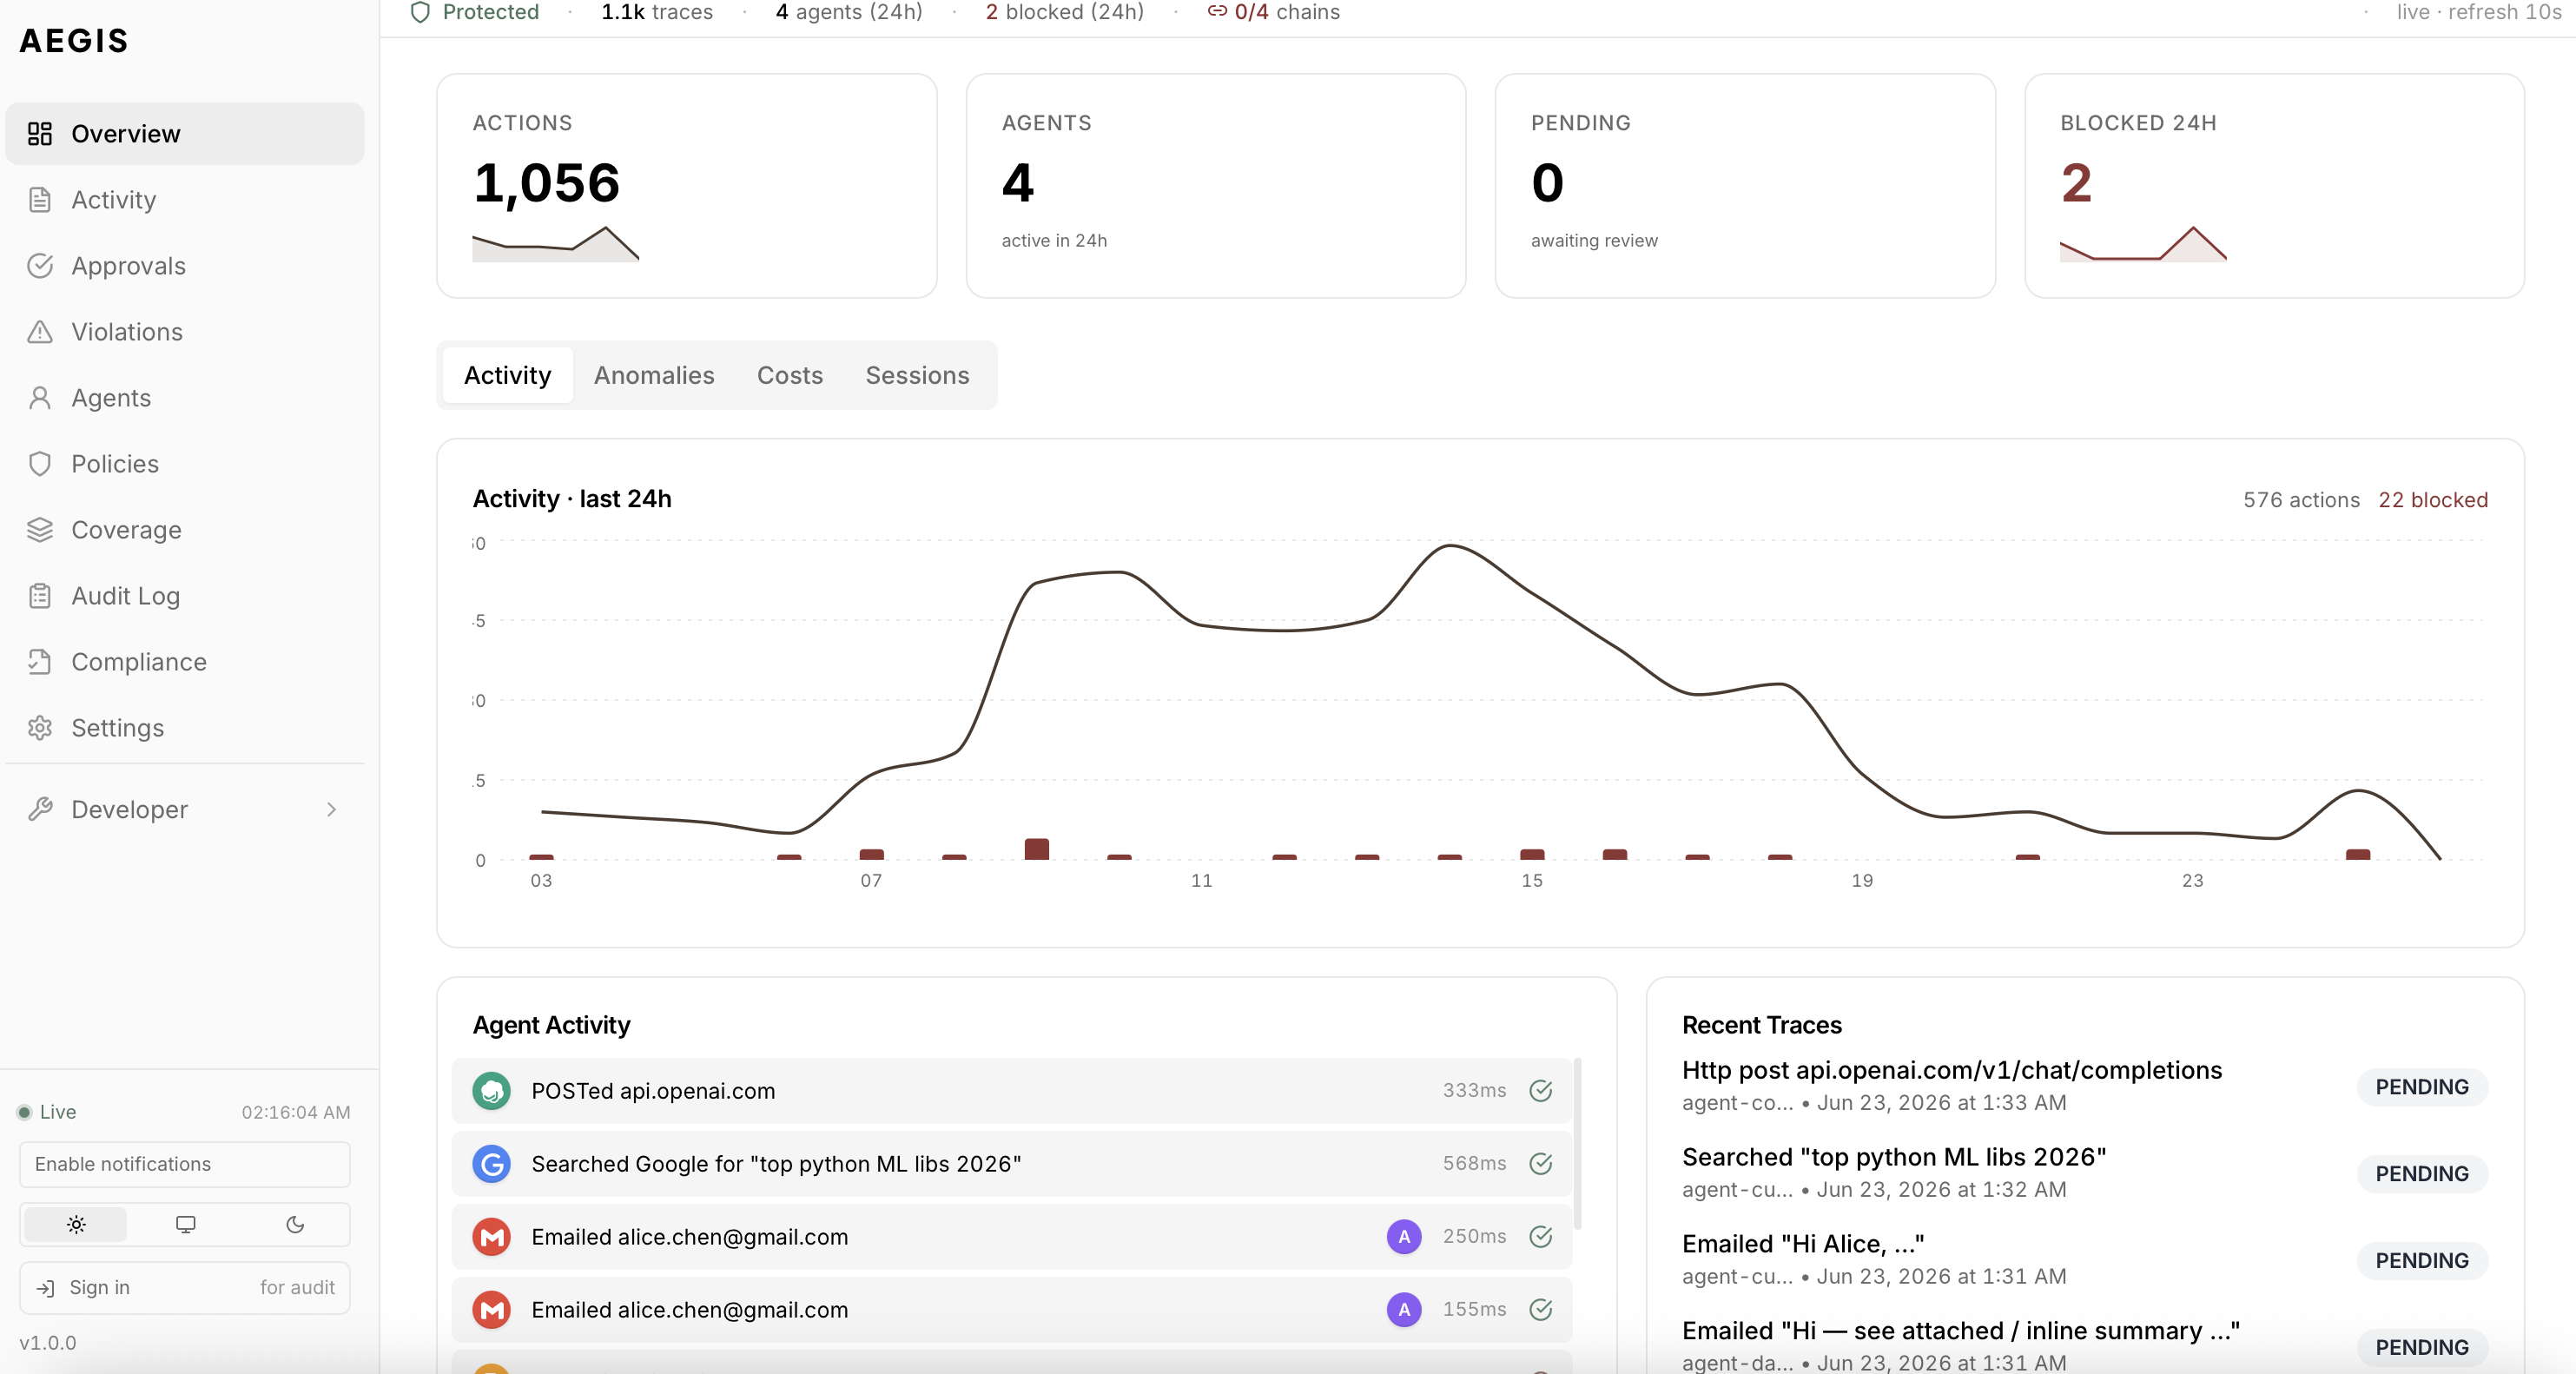
\includegraphics[width=0.98\textwidth]{figures/cockpit_overview.png}
    \caption{Overview dashboard. Real-time counters
    (\textsc{actions}, \textsc{agents}, \textsc{pending},
    \textsc{blocked~24h}) with a 24-hour activity histogram
    and side-by-side agent activity + recent-traces feeds. The
    ``\textsc{Protected}'' chip and \texttt{live · refresh 10s}
    indicator confirm the local gateway is intercepting traffic.}
    \label{fig:cockpit-overview}
\end{figure*}

\begin{figure*}[t]
    \centering
    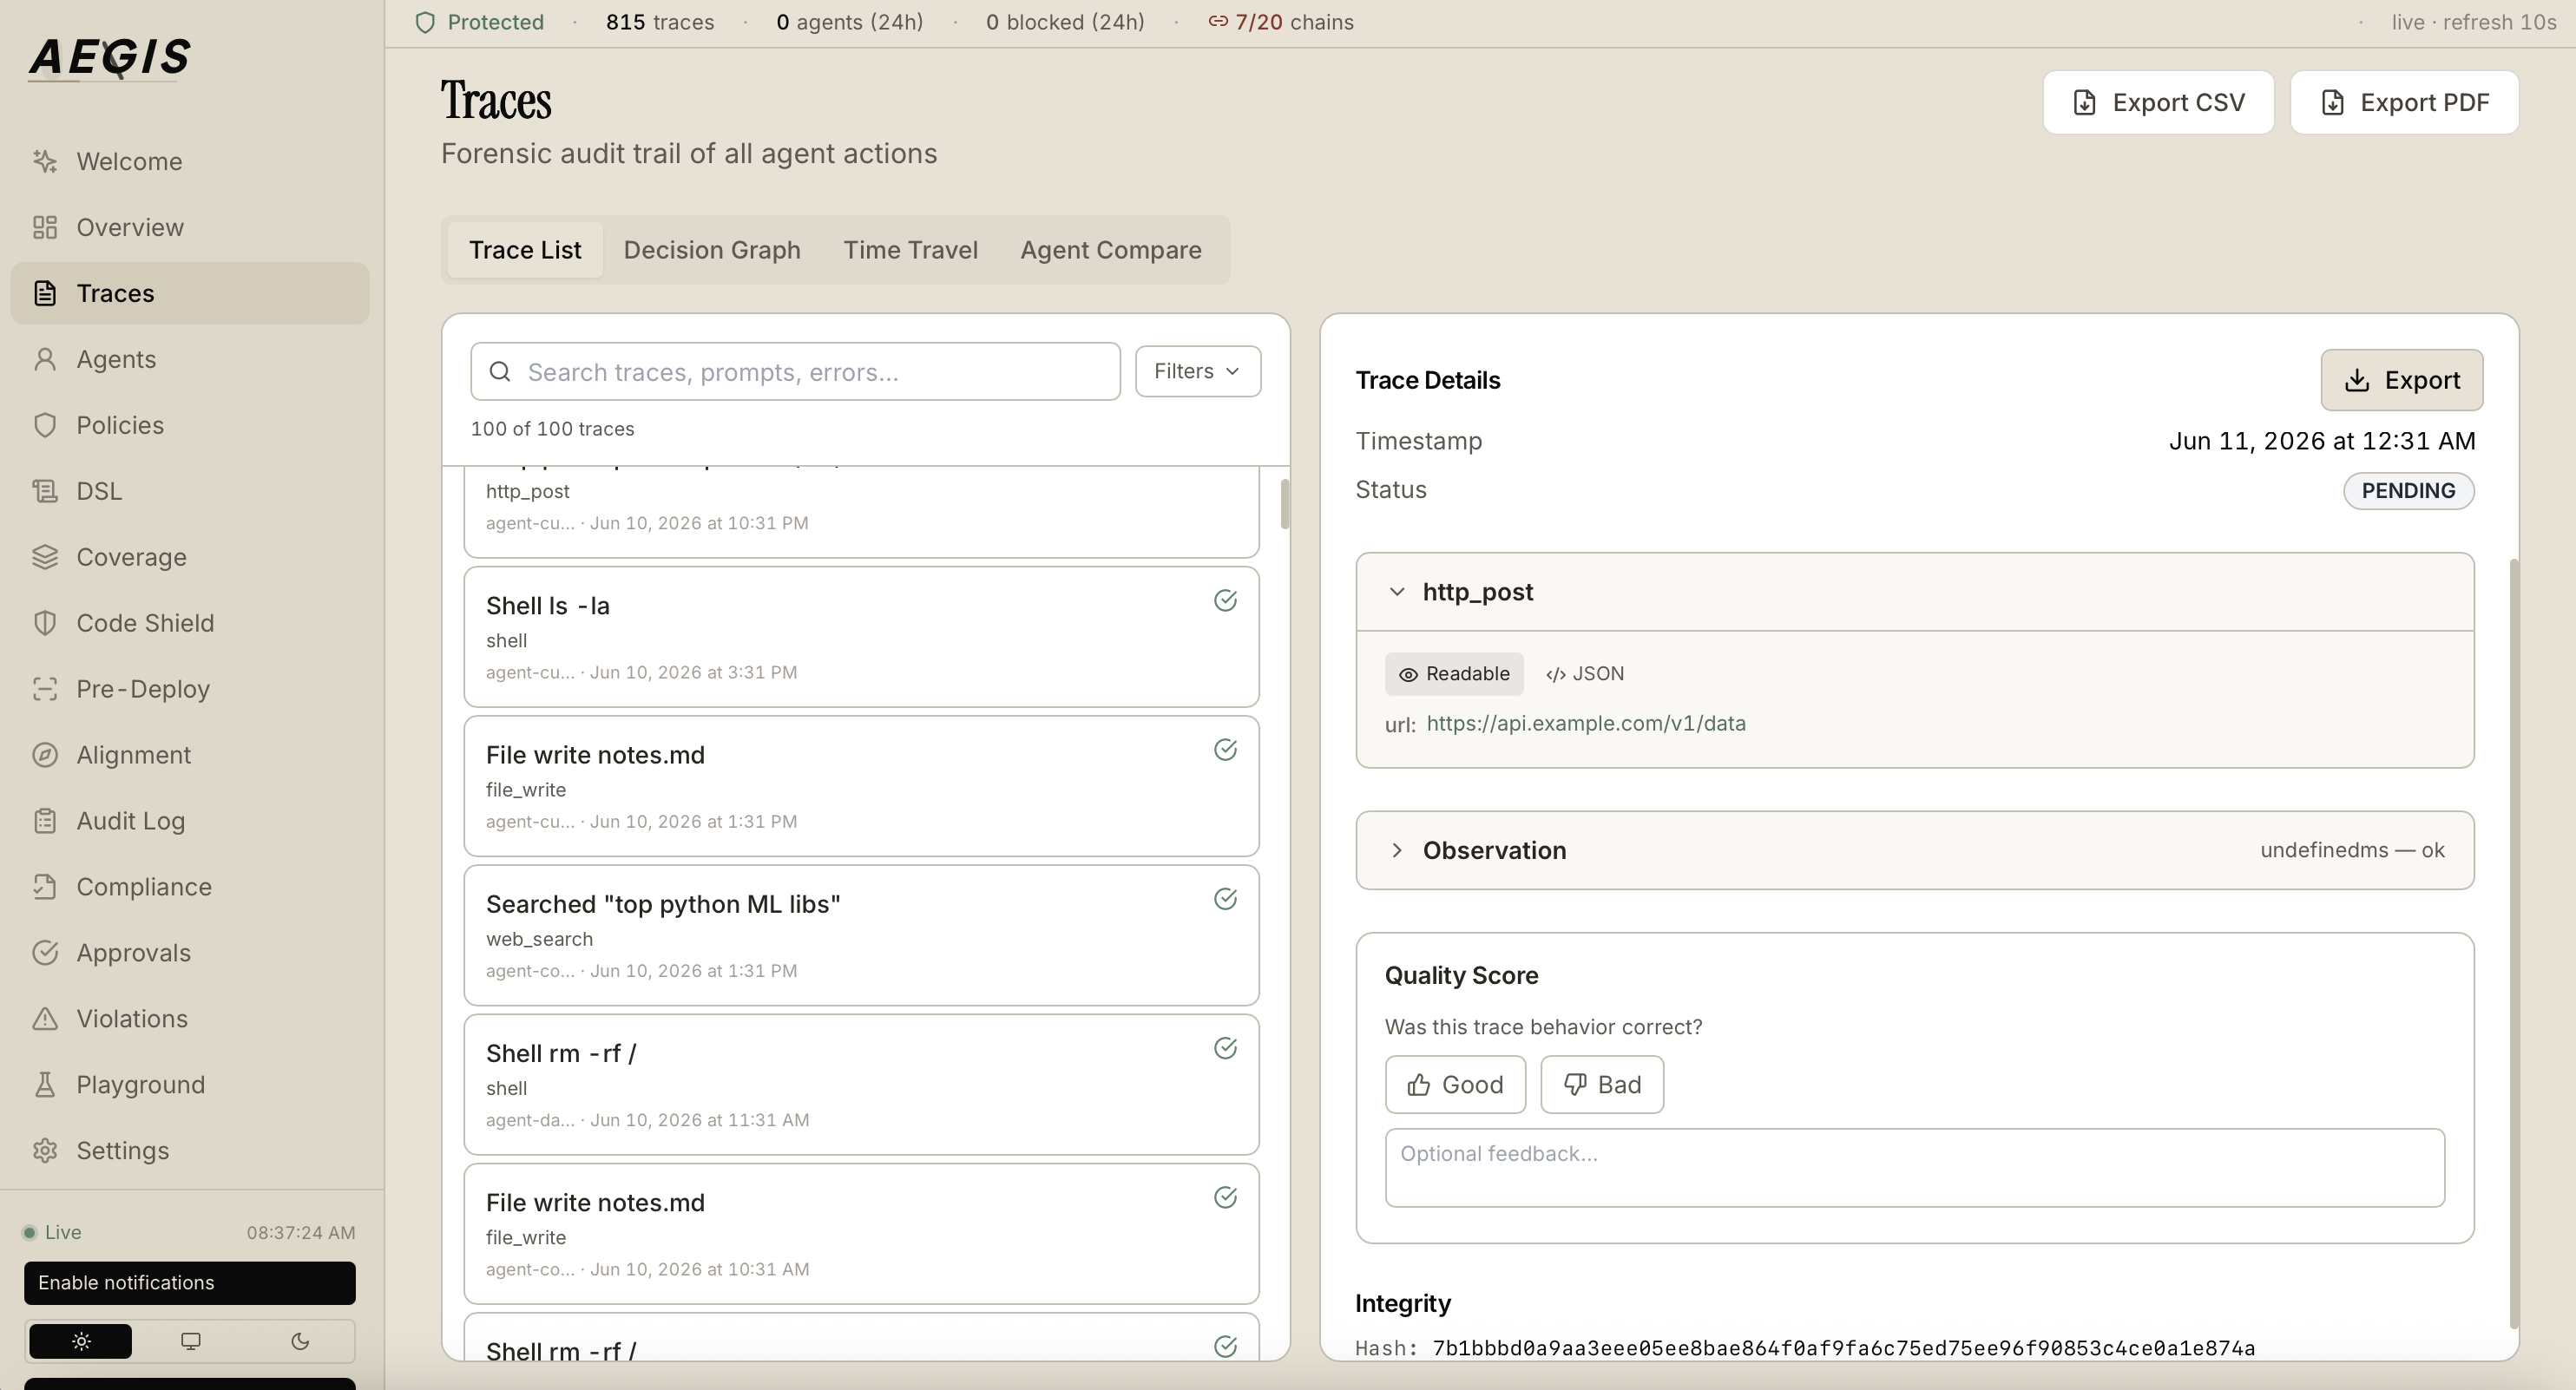
\includegraphics[width=0.98\textwidth]{figures/cockpit_traces-overview.png}
    \caption{Forensic trace explorer. Each row is one \texttt{tool\_use}
    intercepted by the SDK; the right panel expands a single trace
    to show its full argument JSON, cryptographic integrity hash,
    quality-score reviewer buttons, and export controls. Tabs
    (\emph{Trace List}, \emph{Decision Graph}, \emph{Time Travel},
    \emph{Agent Compare}) surface analysis views that are not
    present in observability-only stacks (Langfuse, Helicone, Arize).}
    \label{fig:cockpit-traces}
\end{figure*}

\begin{figure*}[t]
    \centering
    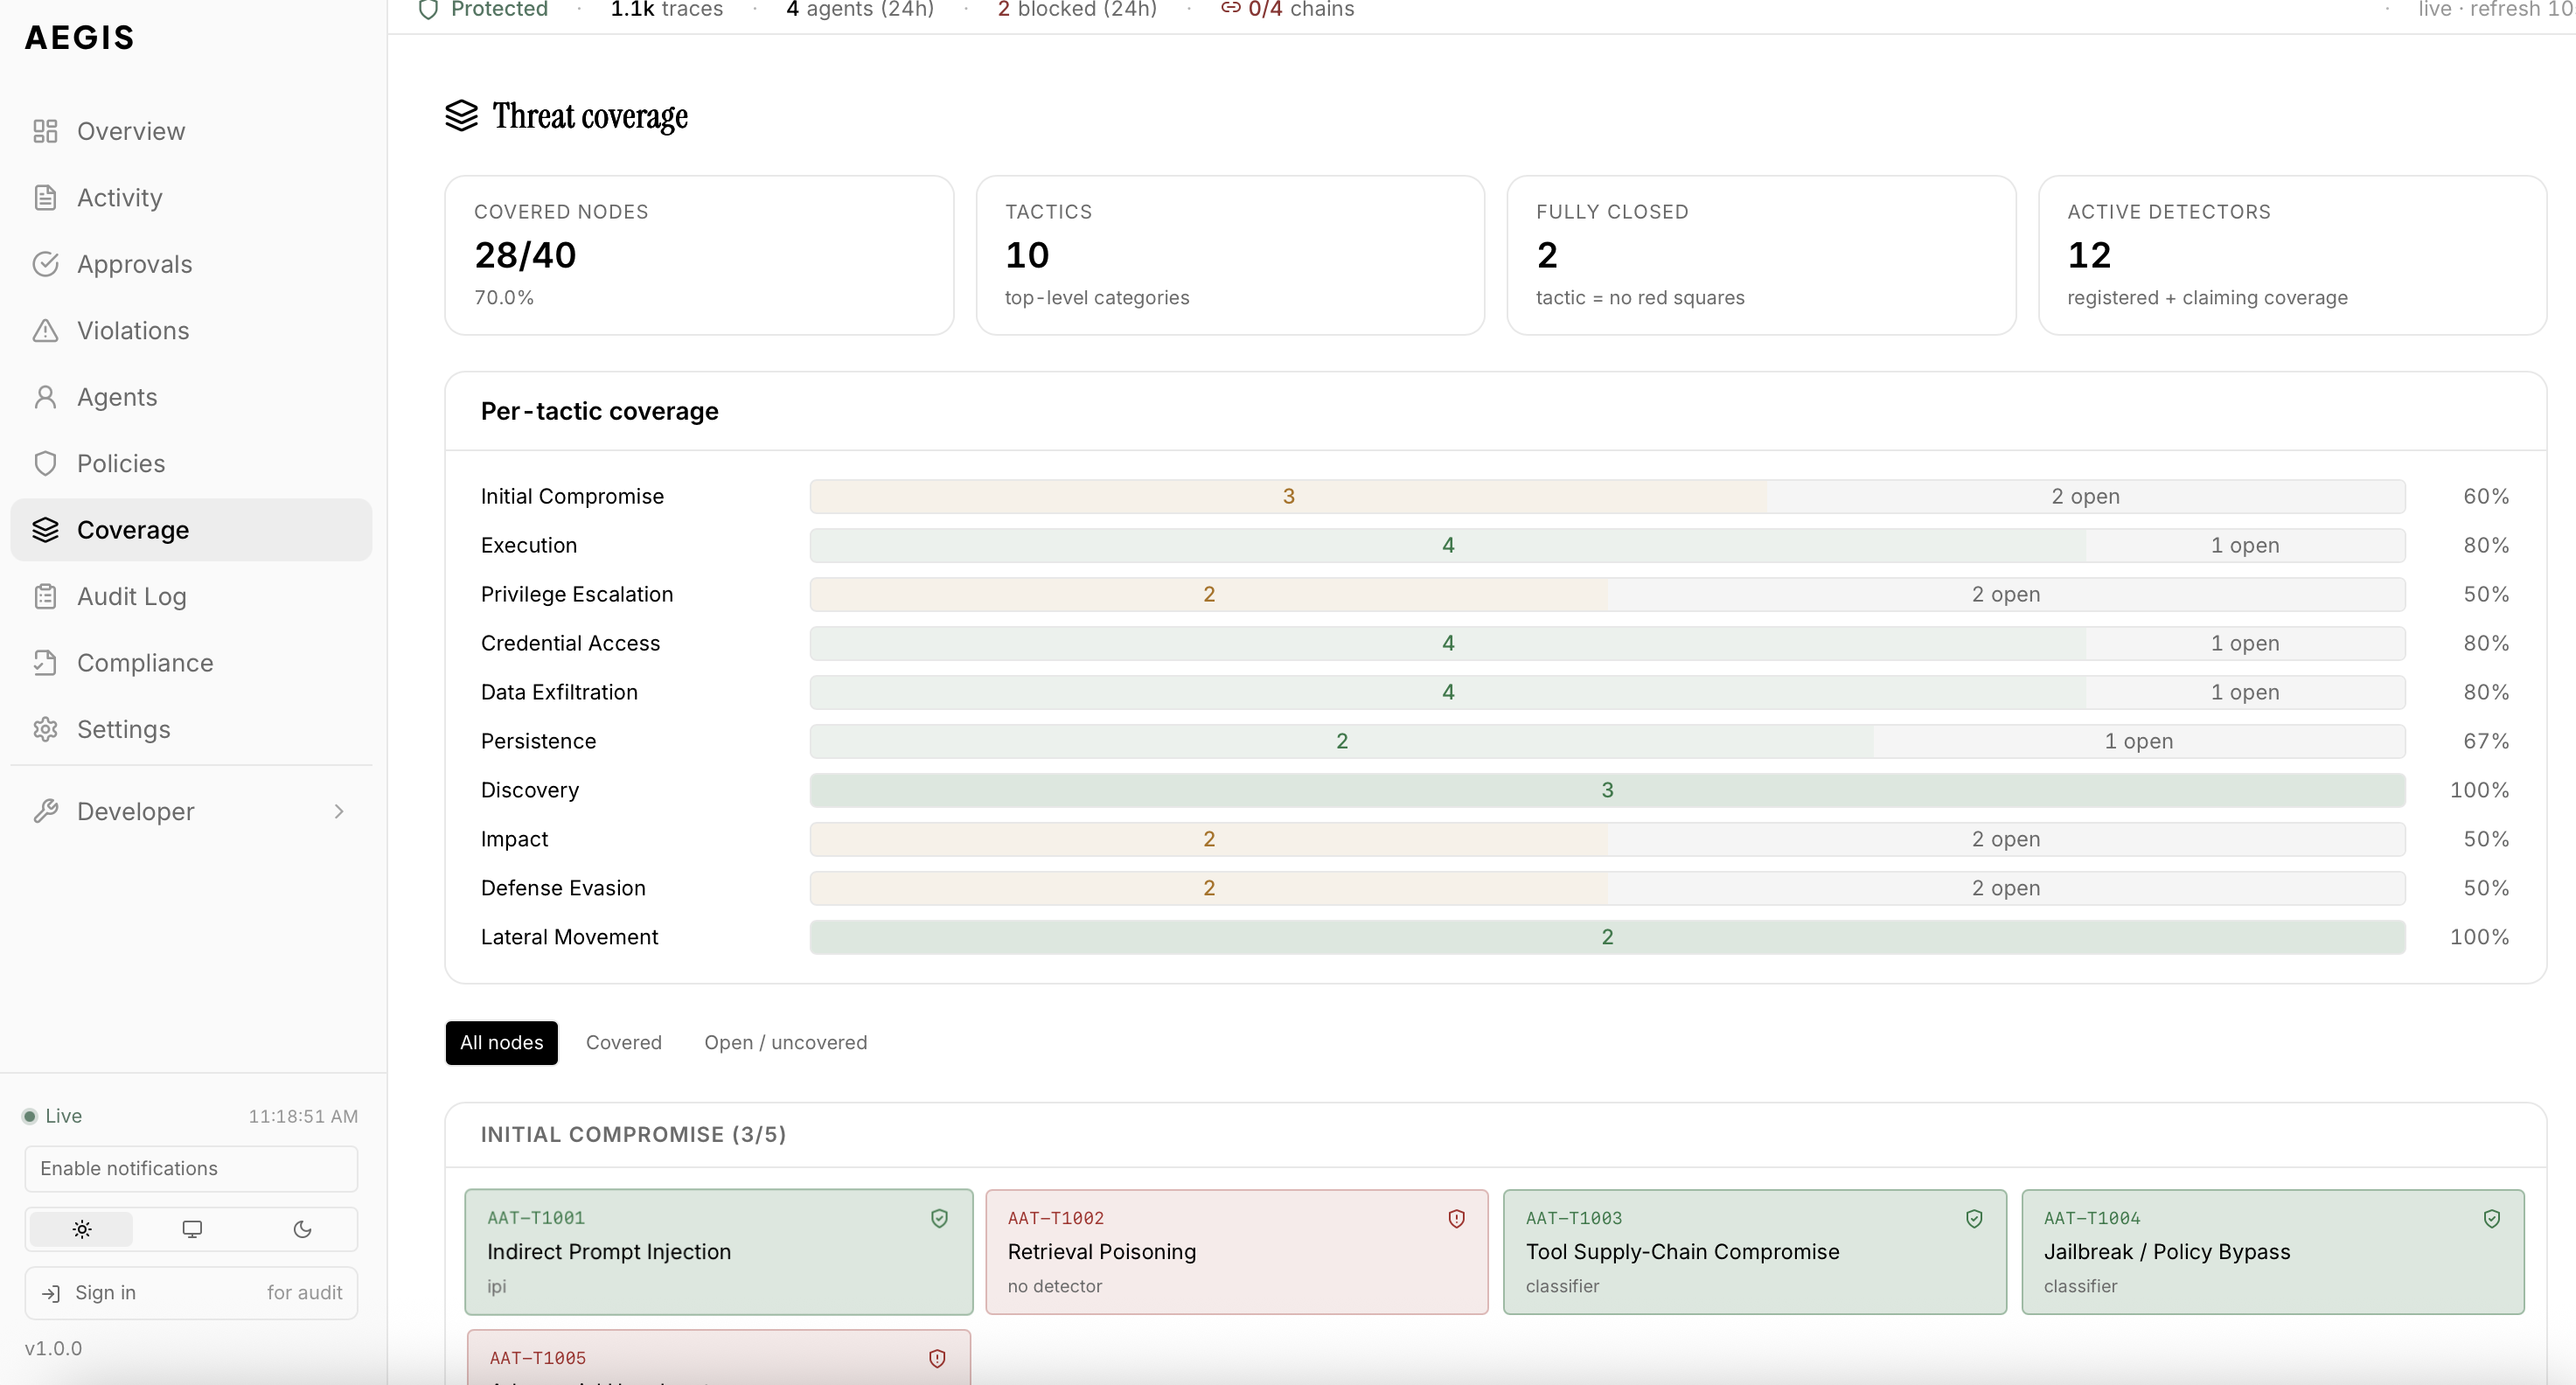
\includegraphics[width=0.98\textwidth]{figures/cockpit_coverage.png}
    \caption{Threat-coverage view (AI Agent ATT\&CK-style taxonomy).
    Ten tactics with per-tactic detector coverage
    (\emph{Initial Compromise}, \emph{Execution},
    \emph{Privilege Escalation}, \emph{Credential Access},
    \emph{Data Exfiltration}, \emph{Persistence}, \emph{Discovery},
    \emph{Impact}, \emph{Defense Evasion}, \emph{Lateral Movement}).
    Green segments are detected, beige are open; the bottom cards
    enumerate specific techniques (AAT-T1001 Indirect Prompt Injection,
    T1002 Retrieval Poisoning, T1003 Tool Supply-Chain Compromise,
    T1004 Jailbreak/Policy Bypass, \ldots) with per-technique detector
    state. This addresses the ``What am I not catching?'' question
    that pure block-rate metrics cannot.}
    \label{fig:cockpit-coverage}
\end{figure*}

\begin{figure*}[t]
    \centering
    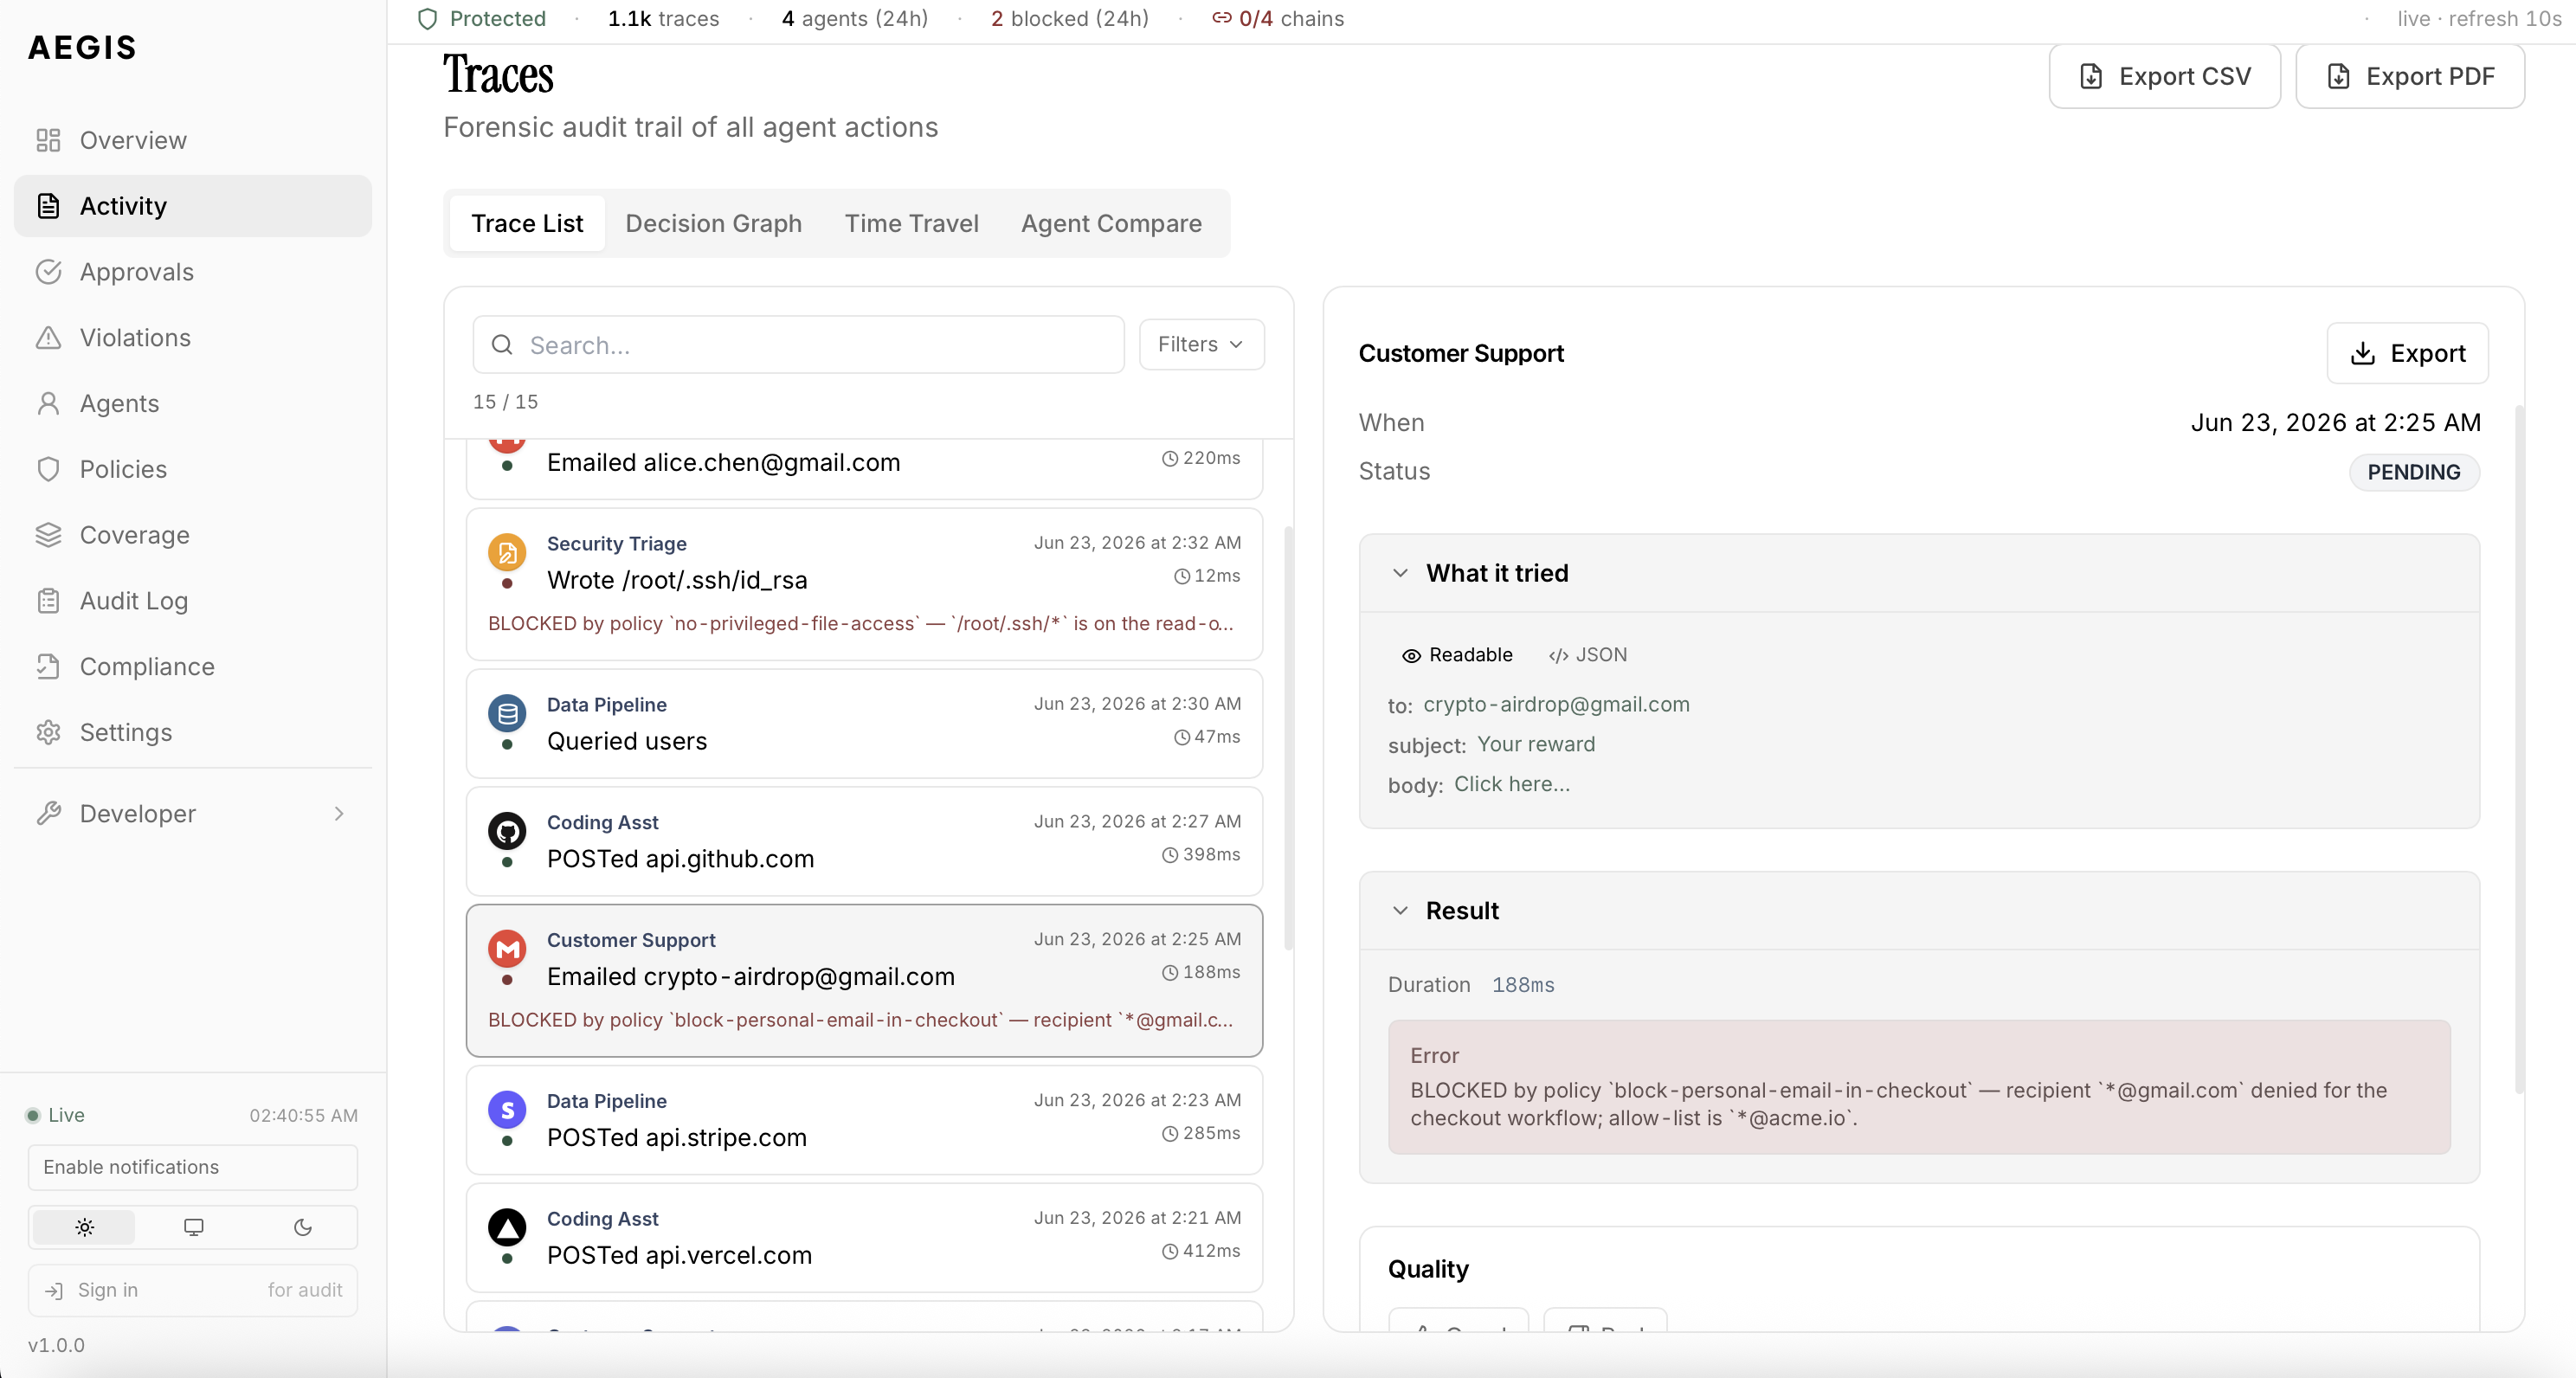
\includegraphics[width=0.98\textwidth]{figures/cockpit_activity.png}
    \caption{Activity feed. Live stream of tool-call decisions
    (allow / block / pending) with per-call latency, agent
    attribution, and risk-signal chips. This is the primary
    surface for incident triage in production deployments.}
    \label{fig:cockpit-activity}
\end{figure*}

\begin{figure*}[t]
    \centering
    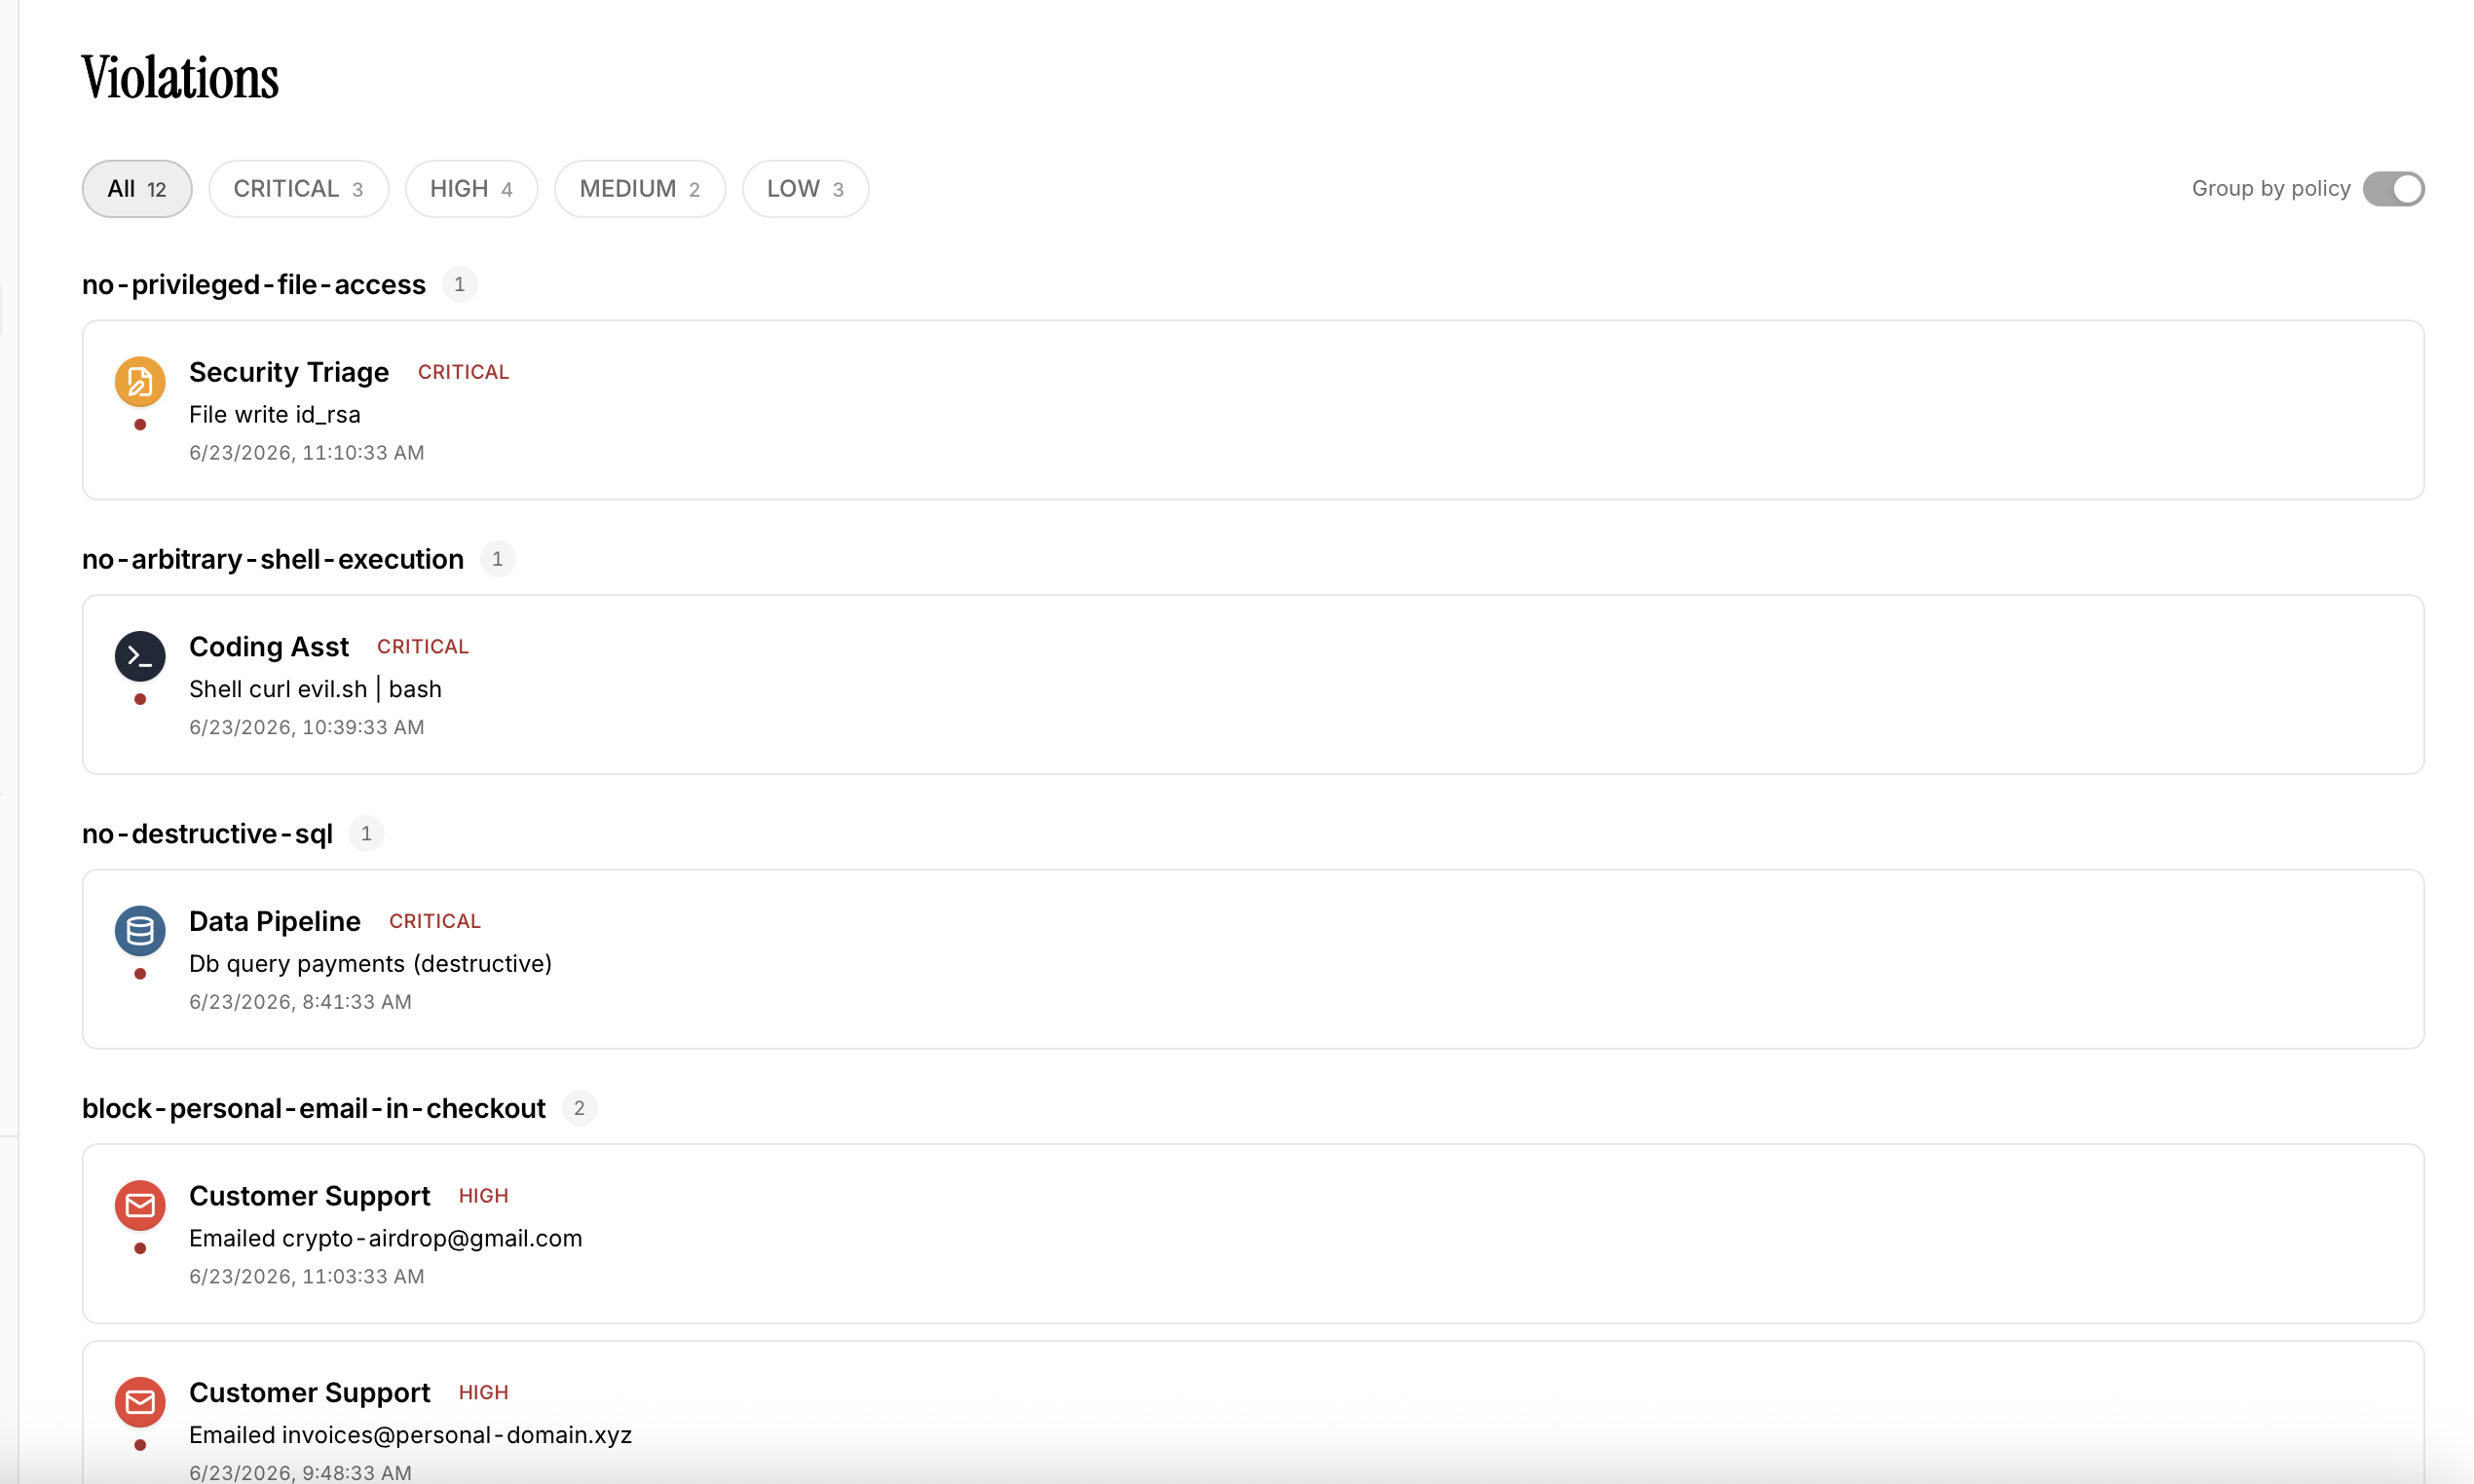
\includegraphics[width=0.98\textwidth]{figures/cockpit_violation.png}
    \caption{Violations panel. Policy violations grouped by
    severity (\textsc{CRITICAL / HIGH / MEDIUM / LOW}) with
    per-agent breakdown and detail expansions. Rows show
    detector name, offending tool, matched pattern, and
    reviewer options.}
    \label{fig:cockpit-violations}
\end{figure*}

\begin{figure*}[t]
    \centering
    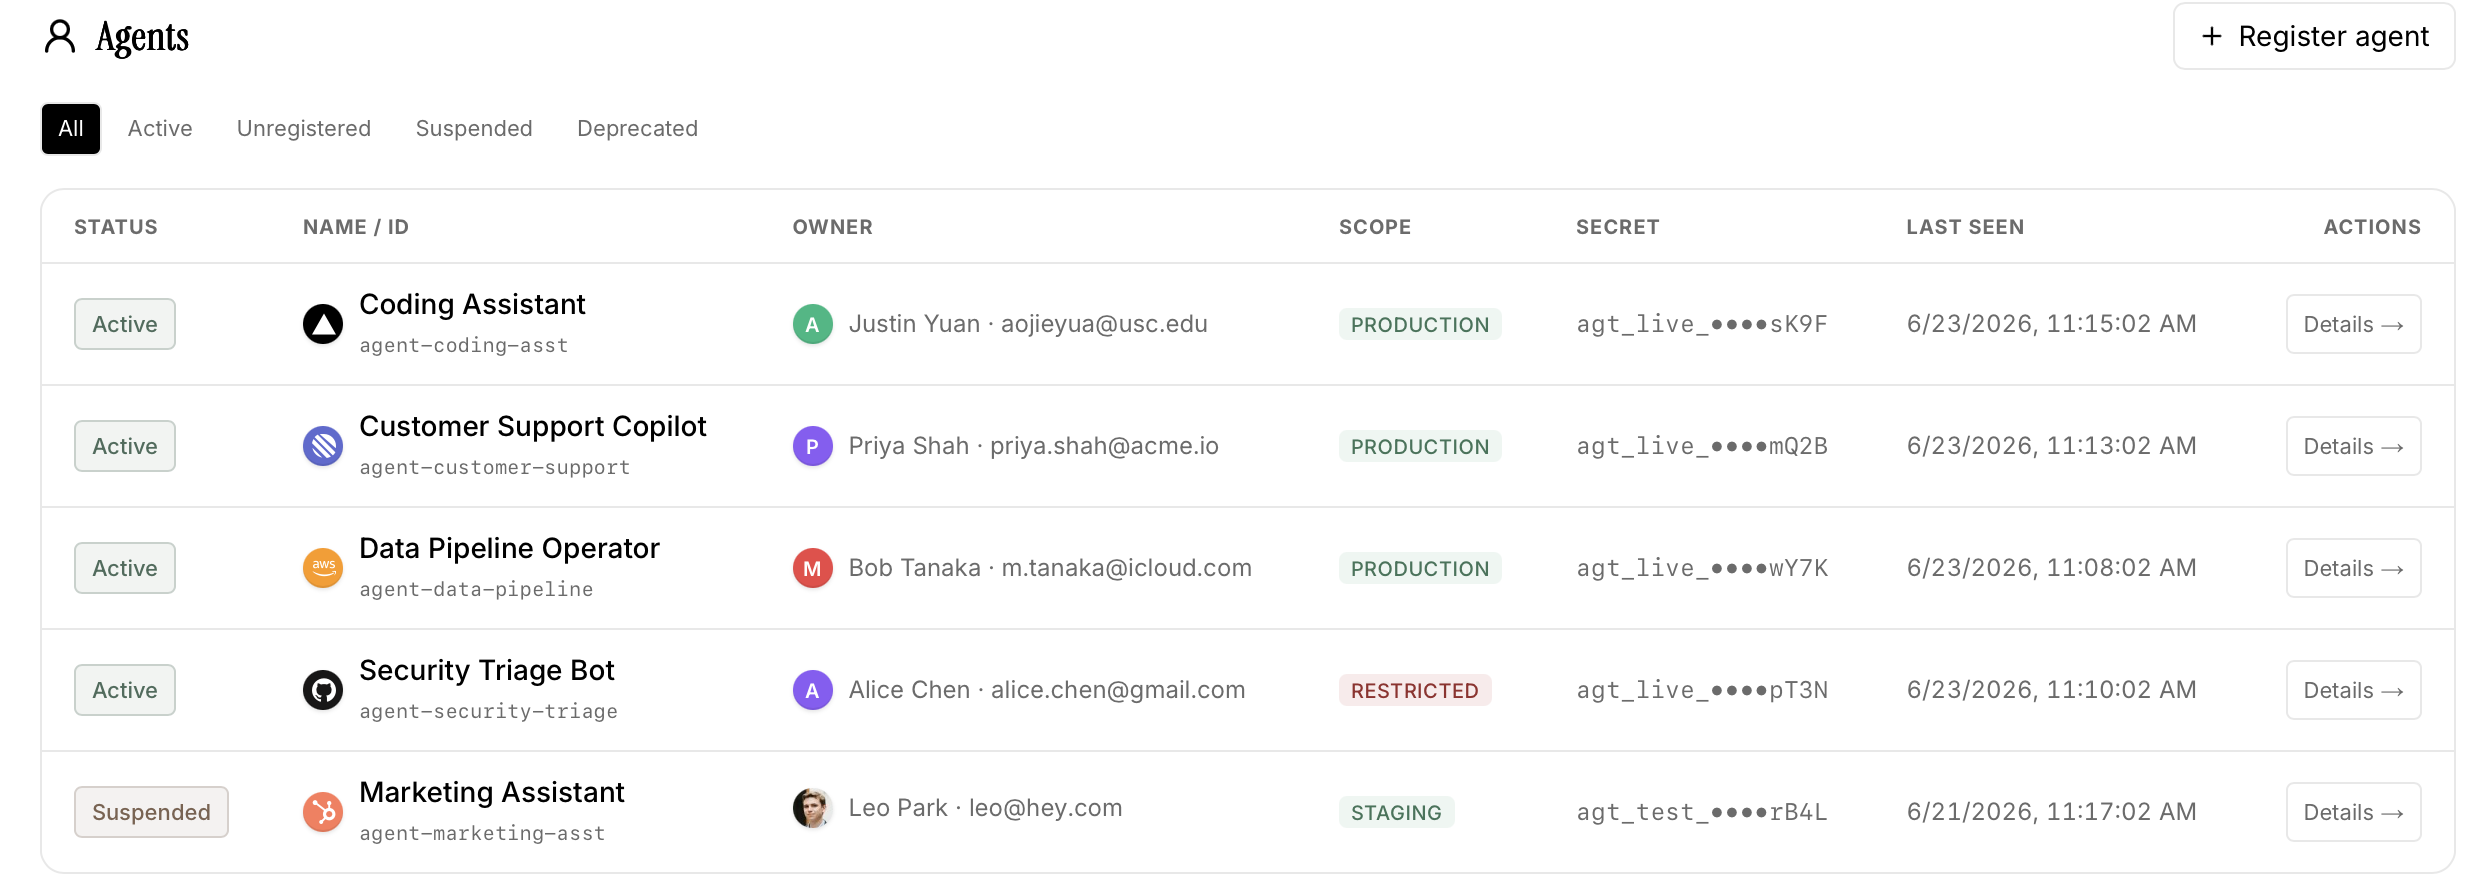
\includegraphics[width=0.98\textwidth]{figures/cockpit_agents.png}
    \caption{Agent registry. Each registered agent carries a
    stable identifier, active-in-24h status, per-agent policy
    scope, and behavioral baseline used for the anomaly-detection
    signal shown in Figure~\ref{fig:cockpit-activity}.}
    \label{fig:cockpit-agents}
\end{figure*}

\begin{figure*}[t]
    \centering
    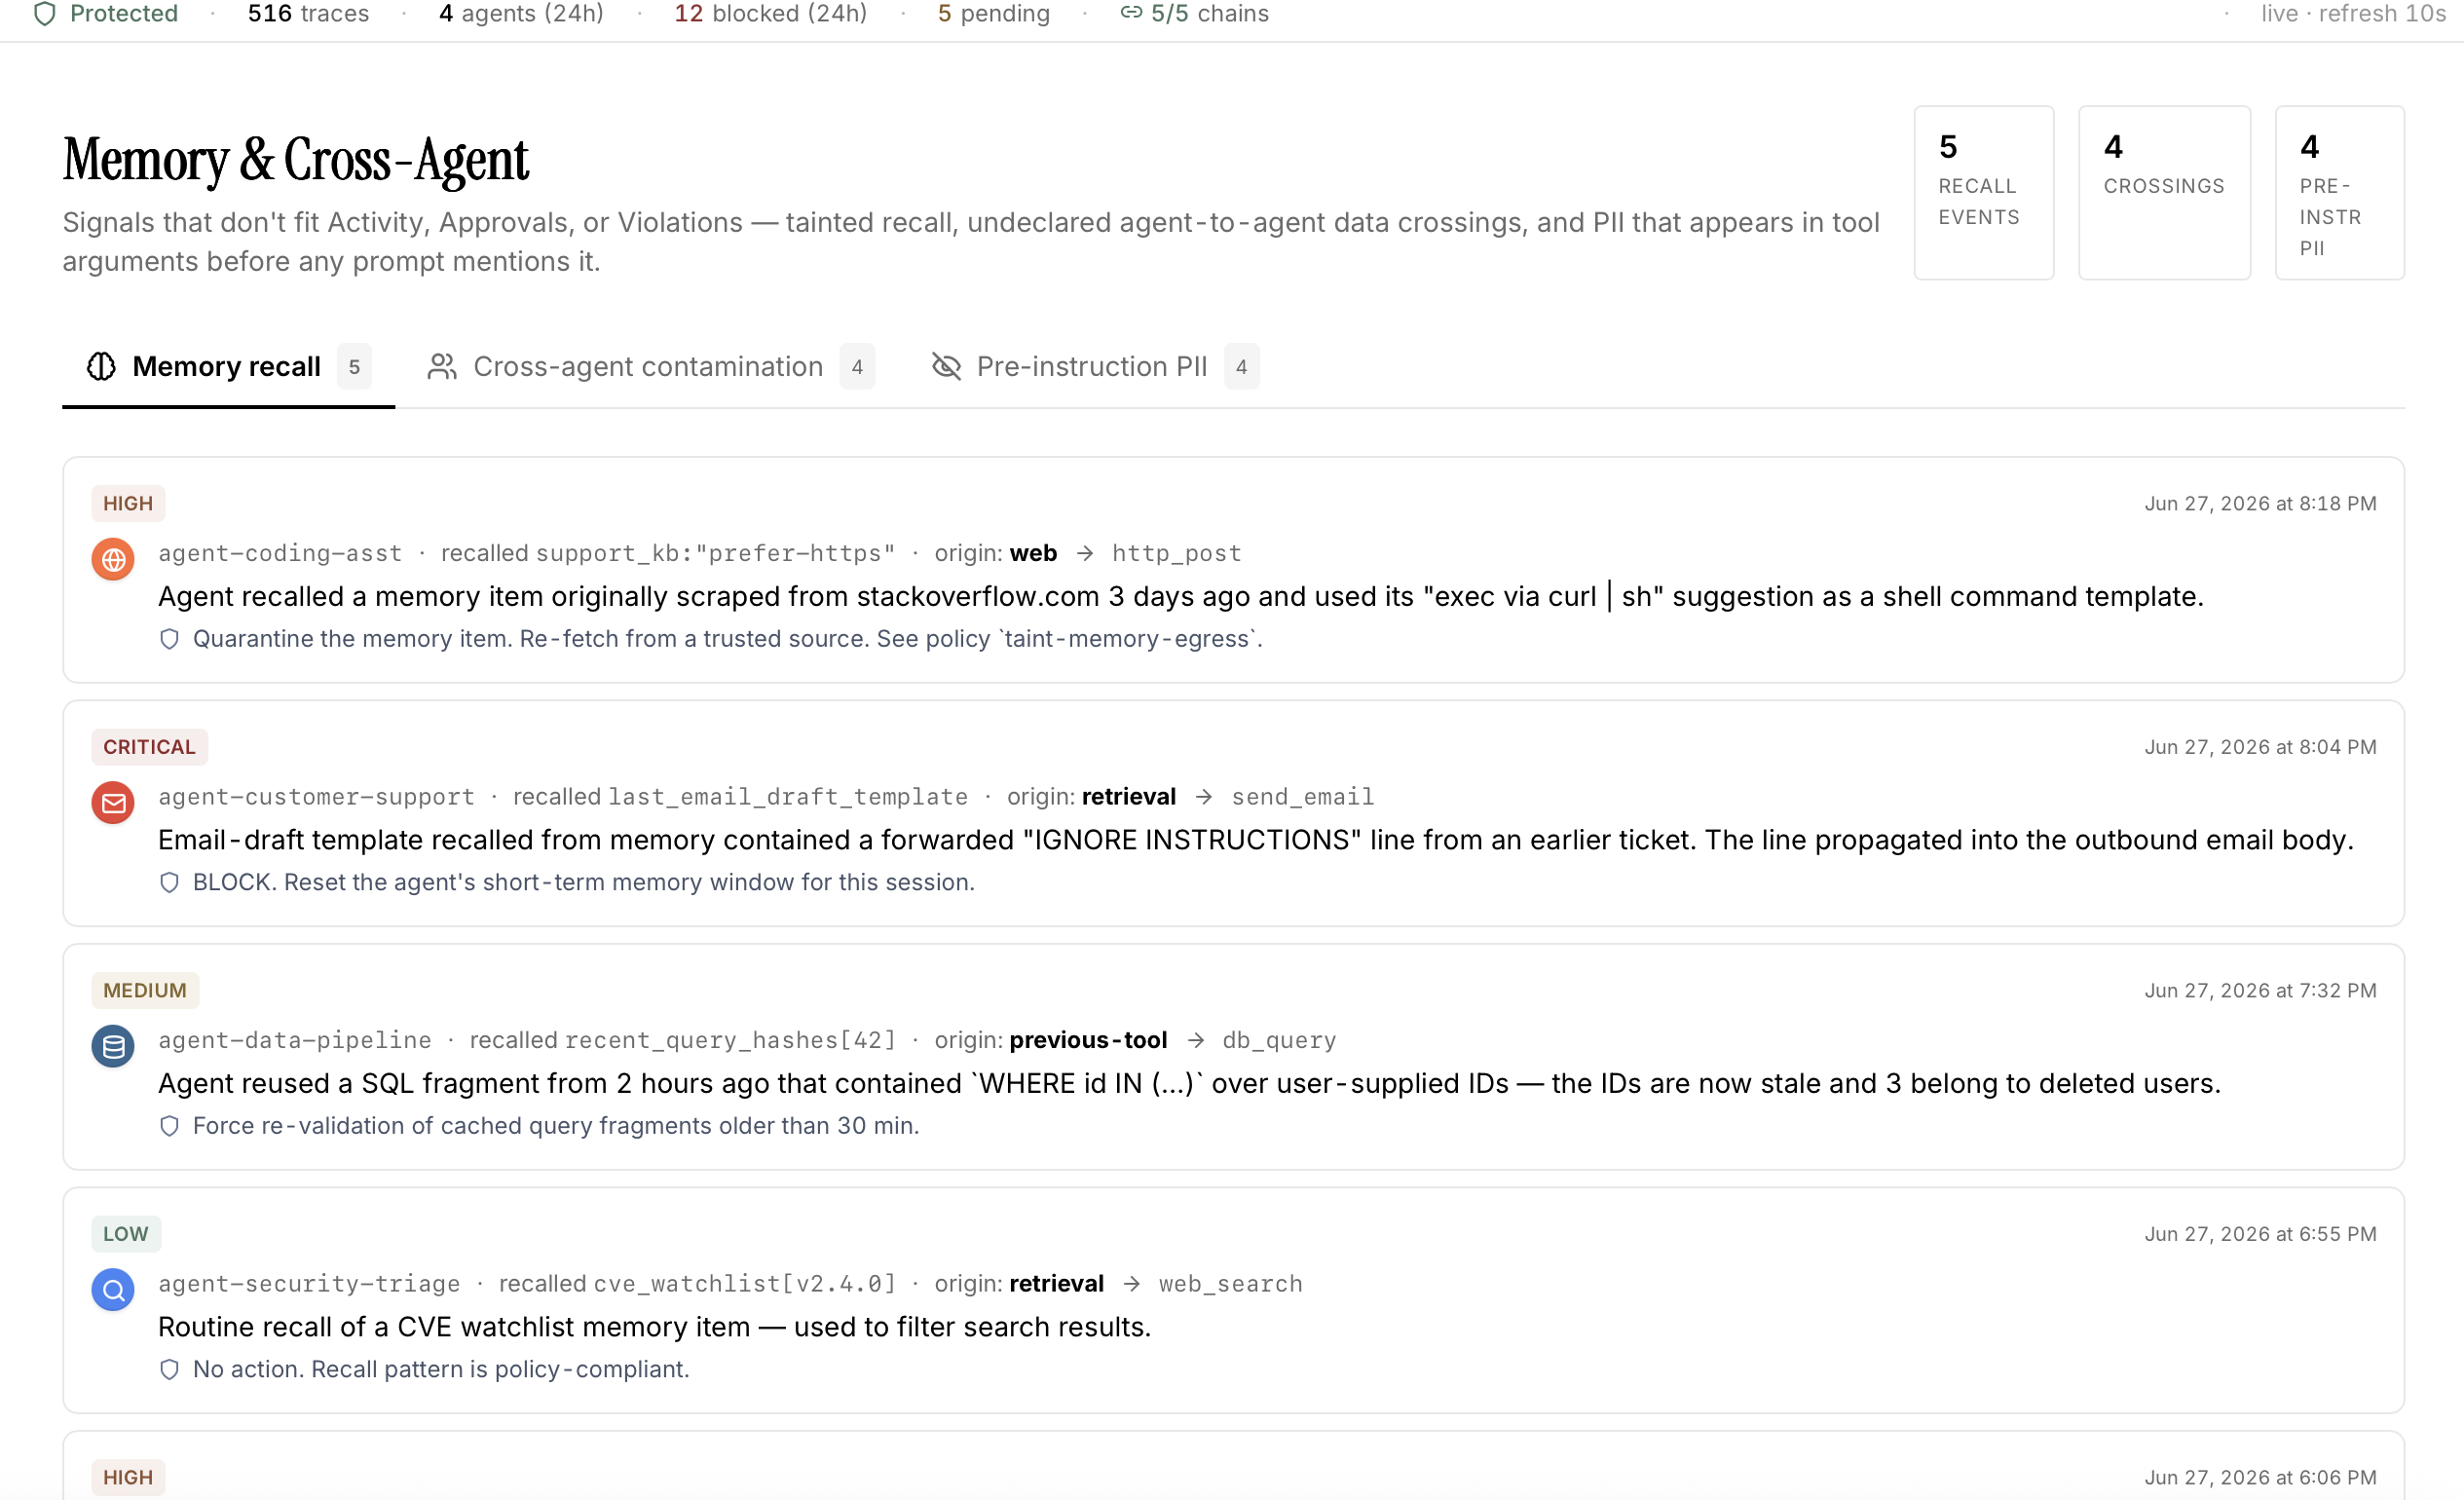
\includegraphics[width=0.98\textwidth]{figures/cockpit_memory.png}
    \caption{Memory / session view. Tool-call sequences grouped
    by \texttt{session\_id} give the reviewer a full workflow
    perspective (which prompt started the chain, which tools
    were called in what order, and at what aggregate cost) rather
    than isolated per-call context.}
    \label{fig:cockpit-memory}
\end{figure*}

\clearpage

% ────────────────────────────────────────────────────────────────
\section{Extended Baseline Comparison}
\label{app:baselines}

Table~\ref{tab:baseline-full} reports every baseline we ran on the
5{,}525-record unified \textsc{ToolGuard-Bench} (a superset of the
\textsc{aegis\_self} v1 suite, InjecAgent, ToolEmu, and OWASP
LLM Top-10 payloads). Figure~\ref{fig:pareto} places these baselines
on the latency--coverage plane. Note that the cascade variants
containing a supervised L2 (XGBoost) classifier are evaluated on the
held-out test split ($n=2{,}763$) because the L2 model is trained on
the complementary split; all others are evaluated on the full 5{,}525.

\begin{table*}[t]
\centering\small
\setlength{\tabcolsep}{4pt}
\begin{tabular}{lrrrrrr}
\toprule
\textbf{Baseline} & $n$ & \textbf{Block \%} & \textbf{FP \%}
                  & \textbf{P50 (ms)} & \textbf{P95 (ms)}
                  & \textbf{Cost} \\
\midrule
No defense                              & 5525 &   0.0 &  0.00 &    0.00 &    0.00 & \$0.00 \\
Keyword blacklist                       & 5525 &   2.5 &  0.00 &    0.00 &    0.01 & \$0.00 \\
\system{}-rules only (arXiv v1)         & 5525 &   1.2 &  0.00 &    0.69 &    1.69 & \$0.00 \\
Llama-Guard 3-8B                        & 5525 &  67.1 &  0.05 &   73.23 &  105.74 & \$0.00 \\
LLM judge (GPT-4o-mini)                 & 5525 &  98.8 & 11.88 & 1203.82 & 1802.60 & \$0.36 \\
LLM judge (Claude Haiku~4.5)            & 5525 &  96.6 &  0.00 & 2211.20 & 3058.50 & \$5.32 \\
Cascade (rules + Haiku, \textbf{no XGB})& 4469 &   4.6 &  6.06 &    5.51 &    6.49 & \$0.17 \\
\textbf{Cascade + XGB (no LLM)}         & 2763 &  \textbf{99.8} &  0.09 & \textbf{0.82} & 1.17 & \textbf{\$0.00} \\
\textbf{Cascade + XGB + Haiku}          & 2763 &  \textbf{99.9} &  0.09 & 1.06 & 2.99 & \$0.05 \\
Cascade + XGB + GPT-4o                  & 2763 &  99.9 &  0.09 & 1.13 & 3.52 & \$0.07 \\
\bottomrule
\end{tabular}
\caption{Baselines on \textsc{ToolGuard-Bench} (5{,}525 records =
3{,}413 malicious + 2{,}112 benign, drawn from InjecAgent, ToolEmu,
OWASP LLM Top-10, and the \textsc{aegis\_self} v1 curated suite).
Cost is total spend on the whole benchmark. \textbf{Cascade + XGB
(no LLM)} matches the LLM-only judges at $10^3\times$ lower latency
and \$0 cost. Adding an LLM layer on top adds $\le$0.1\% coverage
and \$0.05 in aggregate.}
\label{tab:baseline-full}
\end{table*}

\begin{figure*}[t]
    \centering
    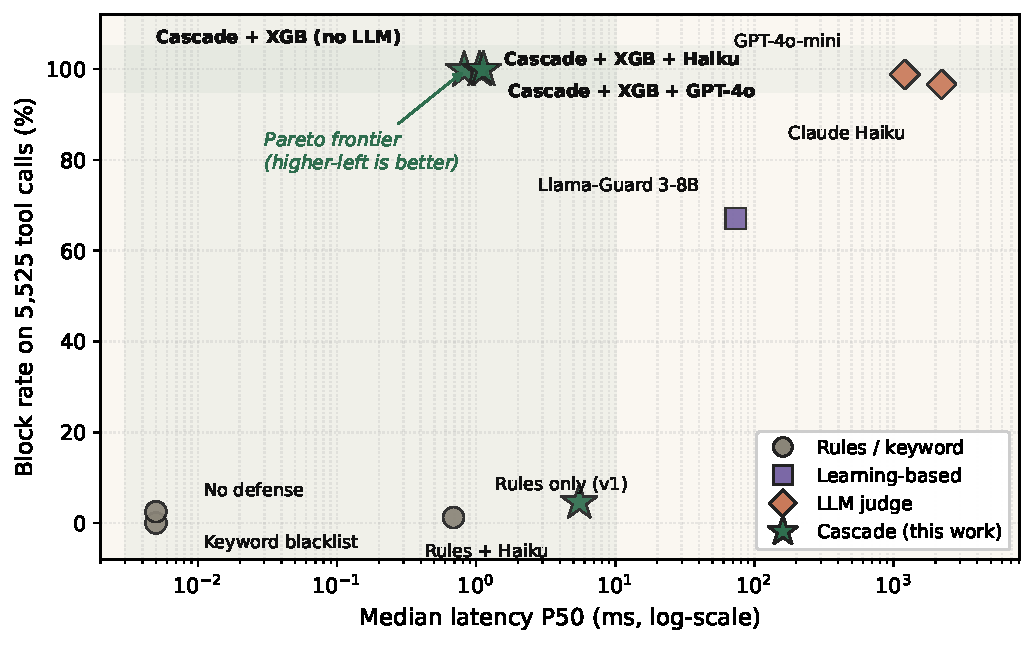
\includegraphics[width=0.90\textwidth]{figures/latency_coverage_pareto.pdf}
    \caption{Latency--coverage Pareto plane on \textsc{ToolGuard-Bench}.
    Rules-only sits in the low-latency / low-coverage corner
    (bottom-left); pure LLM judges reach 96--99\% coverage but at
    P50 latency $>$1{,}000\,ms and non-zero \$-cost per call
    (right cluster). The three \emph{Cascade + XGB} variants
    (upper-left) achieve $>$99\% block rate at $<$1.5\,ms P50 and
    near-zero cost.}
    \label{fig:pareto}
\end{figure*}

\clearpage

% ────────────────────────────────────────────────────────────────
\section{Ablation: Per-Stage Contribution}
\label{app:ablation}

Figure~\ref{fig:ablation} and Table~\ref{tab:ablation} isolate
each stage of the three-layer cascade to answer the
``\emph{is the pipeline non-redundant?}'' question.

\begin{table}[h]
\centering\small
\setlength{\tabcolsep}{4pt}
\begin{tabular}{lrrrr}
\toprule
\textbf{Configuration} & \textbf{Block \%} & \textbf{FP \%} & \textbf{P50} & \textbf{Cost} \\
\midrule
L2 XGB only            &  0.7 & 6.06 & 4.06 & \$0.00 \\
L1 rules + L3 Haiku (no XGB) & 4.6 & 6.06 & 5.51 & \$0.17 \\
L1 rules + L2 XGB (no LLM)   & \textbf{99.8} & 0.09 & 0.82 & \textbf{\$0.00} \\
L1 + L2 XGB + L3 Haiku (full) & \textbf{99.9} & 0.09 & 1.06 & \$0.05 \\
\bottomrule
\end{tabular}
\caption{Per-stage ablation. The L1$\to$L3 cascade \emph{without}
the trained L2 classifier caps at 4.6\% block rate --- the arXiv v1
result. Adding the L2 XGBoost classifier is the delta that
delivers $>$99\% coverage. L3 (LLM judge) adds an incremental
$+0.1\%$ and is only invoked when L2 is uncertain.}
\label{tab:ablation}
\end{table}

\begin{figure}[h]
    \centering
    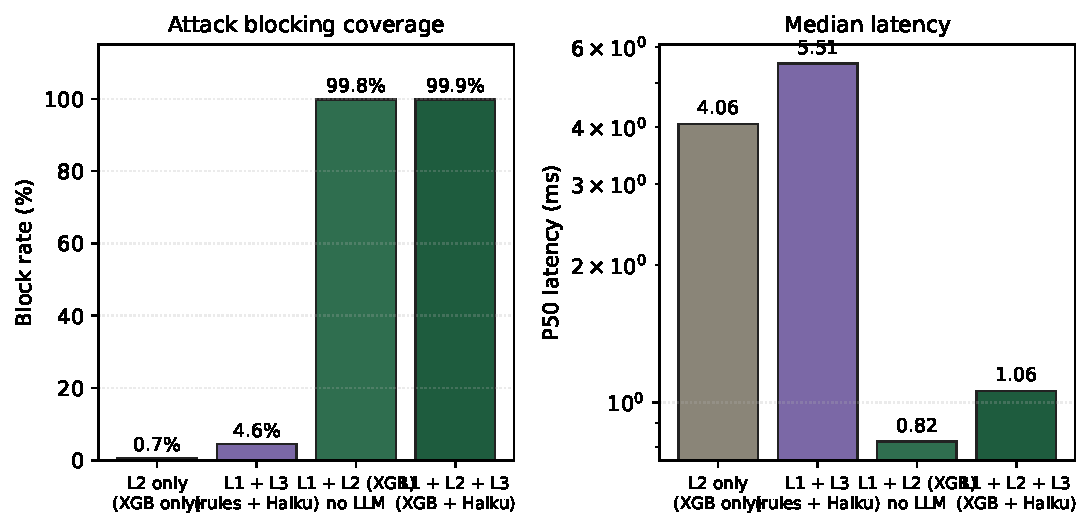
\includegraphics[width=0.98\columnwidth]{figures/ablation_stages.pdf}
    \caption{Per-stage ablation. Block rate (left, linear scale) and
    P50 latency (right, log scale). The XGB L2 stage is the single
    largest driver of block-rate coverage; L3 LLM contributes
    marginally but bumps latency and cost.}
    \label{fig:ablation}
\end{figure}

% ────────────────────────────────────────────────────────────────
\section{Adversarial Robustness}
\label{app:obfuscation}

We stress-tested the cascade against ten obfuscation transforms
applied to the 3{,}413 malicious records, producing an adversarial
benchmark of $3{,}413 \times 10 = 32{,}829$ transformed records
(one transform failed to apply cleanly).

\begin{table}[h]
\centering\small
\begin{tabular}{lr}
\toprule
\textbf{Obfuscation transform} & \textbf{Block \%} \\
\midrule
\texttt{hex\_payload}       & 100.00 \\
\texttt{paraphrase\_prompt} &  99.74 \\
\texttt{sql\_comment\_split}&  99.71 \\
\texttt{unicode\_homoglyph} &  99.09 \\
\texttt{base64\_wrap}       &  99.06 \\
\texttt{whitespace\_pad}    &  98.65 \\
\texttt{double\_url\_encode}&  98.27 \\
\texttt{url\_encode}        &  98.27 \\
\texttt{case\_flip}         &  97.48 \\
\midrule
\textbf{Mean (transforms)}  & \textbf{98.92} \\
\bottomrule
\end{tabular}
\caption{Adversarial robustness of the \emph{Cascade + XGB + Haiku}
pipeline against ten obfuscation transforms on 3{,}413 malicious
InjecAgent records each. Even the weakest transform
(\texttt{case\_flip}) is caught 97.5\% of the time, and no
transform drops below 97\%.}
\label{tab:obfuscation}
\end{table}

% ────────────────────────────────────────────────────────────────
\section{SDK Integration Reference}
\label{app:sdk}

For completeness, Listing~\ref{lst:python-integration} shows the
Python integration path shipping in the v0.2.0 release. The
same one-line \texttt{auto()} idiom works across all 14
supported frameworks (9 Python, 4 JS/TS, 1 Go).

\begin{lstlisting}[language=Python,caption={A Claude agent with \system{} protection (three added lines).},label=lst:python-integration]
import anthropic
import agentguard          # <-- add
agentguard.auto()          # <-- add

client = anthropic.Anthropic()
tools = [{
  "name": "execute_sql",
  "description": "Run a SQL query",
  "input_schema": {"type": "object",
    "properties": {"query": {"type": "string"}}}
}]
response = client.messages.create(
    model="claude-sonnet-4-5",
    max_tokens=1024,
    tools=tools,
    messages=[{"role": "user",
               "content": "Show all customers"}])
# AEGIS intercepts tool_use blocks here
# before execute_sql() is called
\end{lstlisting}

% ────────────────────────────────────────────────────────────────
\section{Reproducibility}
\label{app:repro}

All experiments were run against the open-source \system{} build
tagged \texttt{v0.2.0}. The unified benchmark, per-record predictions,
and summary metrics are versioned in the same repository under
\texttt{research/benchmark/data/} and \texttt{research/results/}.
The end-to-end reproduction sequence is:

\begin{lstlisting}[language=bash,basicstyle=\ttfamily\scriptsize]
# 1. Build the unified benchmark from raw sources
python -m research.benchmark.build

# 2. Reproduce Table 1 by running every baseline
python -m research.baselines.run --baseline aegis_rules
python -m research.baselines.run --baseline llama_guard
python -m research.baselines.run --baseline llm_judge_anthropic
python -m research.baselines.run --baseline llm_judge_openai

# 3. Reproduce the cascade + ablation results
python -m research.cascade.run_cascade \
    --L1 1 --L2 xgboost --L3 1

# 4. Reproduce cross-source generalization
python -m research.cascade.run_cross_source
\end{lstlisting}

Each invocation writes a directory
\texttt{results/<baseline>\_\_<bench>\_\_<timestamp>/}
containing \texttt{predictions.jsonl} and \texttt{summary.json}.
Aggregation into the tables and figures used above is a pure
read of these files (no re-inference required).


\end{document}
